\documentclass[preprint,12pt]{elsarticle}
\usepackage[utf8]{inputenc}
\usepackage[T1]{fontenc}
\usepackage{amsmath,amssymb}
\usepackage{graphicx,booktabs,array}
\usepackage[colorlinks=true,allcolors=blue,pageanchor=false]{hyperref}
\usepackage{xurl}
\emergencystretch=3em
\sloppy
\journal{Physics of the Dark Universe}
\begin{document}
\begin{frontmatter}
\title{Density-Dependent Vacuum Bubble Nucleation in Matter-Coupled Dark-Sector Cosmology: Dark-Matter Granularity, Wall Dynamics and Transmission}
\author{Leon Sandler}
\ead{sandler.leon@gmail.com}
\affiliation{organization={Independent Researcher},city={Northbrook},state={Illinois},country={USA}}
\begin{abstract}
Can a declining dark-matter density switch on the decay of a vacuum? For a scalar whose coupling to dark matter is centered on a false vacuum, the mean-field effective potential becomes metastable below a degeneracy density and Coleman--De Luccia tunneling switches on. We test the assumption behind this picture, that the field feels a smooth density. For a vacuum at the dark-energy scale the field's Compton length is approximately 0.07 mm, and the dark-matter energy inside a Compton volume is only 0.05$m_\varphi^4$. A spatially resolved treatment, the static field around discrete sources and the decay rate with randomly placed sources at first order in each source's coupling, shows that particle dark matter leaves the vacuum between the particles at its zero-density rate: for 1 MeV particles a fraction $7\times10^{-8}$ of the mean-field suppression survives. The mean field holds for wave dark matter heavier than the field and still classical, approximately 3 meV to 0.25 eV, which a 1+1-dimensional simulation of a wall running through such dark matter confirms. The decay is then environmental: a region completes its transition at a scale factor proportional to $(1+\delta)^{1/3}$, voids first, while galactic haloes keep the held vacuum. The walls run away; dark matter crossing them gains the sudden-crossing energy and trails the wall at 0.75c. Transitioned regions recollapse, an isolated Hubble-scale bubble develops a trapped surface before its interior bounces, and an optional neutrino coupling would be invisible to terrestrial oscillation experiments.
\end{abstract}
\begin{highlights}
\item Dilution makes a matter-held vacuum metastable below a degeneracy density
\item Resolved tests: with particle dark matter the vacuum decays at its zero-density rate
\item Wave dark matter between 3 meV and 0.25 eV restores the smooth mean field
\item Regions decay in order of their density; galactic haloes keep the old vacuum
\item Dark matter crossing the runaway wall is kicked forward at three quarters of c
\end{highlights}
\begin{keyword}
vacuum decay \sep bubble nucleation \sep coupled dark matter \sep wave dark matter \sep dark energy \sep cosmic voids \sep mass-varying neutrinos
\end{keyword}
\end{frontmatter}



\section{Introduction}
False-vacuum decay proceeds by the nucleation of bubbles of the true vacuum, whose rate follows from the Euclidean bounce [1, 2] and whose gravitational corrections were derived by Coleman and De Luccia [3]. The theory is usually applied to a vacuum whose stability does not depend on its surroundings. In a universe filled with dark matter, however, a scalar that couples to the dark matter feels an effective potential that depends on the dark-matter density, as in chameleon and symmetron screening [4, 5, 6] and in coupled dark energy [7]. If the dark energy is the energy of such a scalar held in a vacuum by the matter term, the dilution of the dark matter by the expansion changes the vacuum structure itself, and the decay of the vacuum is placed under the control of the cosmic density. This paper asks three questions. Can a declining dark-matter density turn a stable vacuum into a metastable one? When is the density that the field feels the smooth mean density that such an argument assumes? And what do the resulting vacuum walls do: what crosses them, how do they move, and what becomes of the region they enclose?

Environment-dependent vacua are familiar from screened modified gravity, where the field's minimum and mass track the local density [4, 5, 6]; in those applications the field's Compton length is long compared with the separation of the matter particles, and the density can be averaged. Vacuum decay out of a metastable state has been studied for vacua whose stability is fixed, from the Standard Model Higgs [8, 9] to landscapes of many vacua [10, 11], including the signatures of bubble collisions [12, 13]. Combining the two raises a question that neither literature had to face: a vacuum at the dark-energy scale has a Compton length below a millimeter, and whether the dark matter looks smooth on that scale depends on what the dark matter is. The interfaces add a further question. A wall between vacua in which the dark-matter mass differs is a mass step; slow walls reflect particles whose momentum is below the step, which has been proposed as a way to filter dark matter at first-order transitions [14], while fast walls transmit them and the pressure they exert is bounded [15, 16]. Bubbles of a negative vacuum enclose regions that recollapse, and bubbles in an expanding exterior can be cut off behind horizons [17, 18, 19].

The contributions are the following. (i) The phase structure of a matter-coupled potential is mapped as a function of density and tilt (Section 2). (ii) The conditions under which the field feels a smooth density are derived and tested with spatially resolved calculations; within them, particle dark matter does not provide a smooth source, and a window remains for wave dark matter heavier than the field, a bound that follows from the dark-energy scale itself (Section 3). (iii) The bounce, the wall and the density-dependent action are computed and validated, and the nucleation history is followed in the emptiest regions, where it begins, with the consequences of the environment for the protection of the past and for the regions that keep the held vacuum (Section 4). (iv) The transmission of fields and of the dark matter through the wall is computed (Section 5), (v) the gravitational dynamics of the wall and the completion of the transition are computed with explicit bounds on the approximations (Section 6), and (vi) the region enclosed by the wall is evolved as a cosmology (Section 7). (vii) Controls that remove the coupling, a viability map and parameter surveys identify where the conditions hold (Section 8), and (viii) an optional coupling of the scalar to neutrinos is examined for its experimental consequences (Section 9).

Units are $\hbar=c=k_B=1$, $M_{\rm Pl}$ is the reduced Planck mass, and every number quoted is read from the output of the script named in parentheses in the archived code. The paper does not require a cosmological bounce. A companion paper treats the symmetron version of the trigger, whose release is a classical roll on cosmological scales, and its continuation into cycles [20]; the two papers share the class of models but not their results.

\section{Matter-coupled vacuum metastability}
A scalar coupled conformally to dark matter has the action

\begin{equation}
S=\int d^4x\sqrt{-g}\left[\frac{M_{\rm Pl}^2R}{2}-\frac{1}{2}(\nabla\varphi)^2-V_0(\varphi)\right]+S_{\rm dm}\left[A^2(\varphi)g_{\mu\nu},\psi_{\rm dm}\right]
\end{equation}
and, where the dark matter can be described by a smooth nonrelativistic density, the conserved Einstein-frame density $\rho_*$ enters the field equation through $V_{\rm eff}(\varphi,\rho_*)=V_0(\varphi)+\rho_*A(\varphi)$ [7, 5]. When this mean-field description holds is the subject of Section 3; here it is assumed. We take the tilted quartic $V_0$ in the dimensionless form

\begin{equation}\begin{gathered}
p(x;\eta,\theta)=\frac{(x^2-1)^2}{8}+\frac{\eta x}{2}+\frac{\theta}{2}(x-1)^2,\qquad x=\frac{\varphi}{f},\\
\theta=\frac{\rho_*}{\lambda f^2M^2},\qquad V_{\rm eff}=\lambda f^4\,p+{\rm const}
\end{gathered}\end{equation}
where $\eta$ tilts the potential so that $x\approx-1$ is the zero-density true vacuum and $x\approx1$ the false one, and the coupling $A(\varphi)=1+(\varphi-f)^2/2M^2$ is centered on the false vacuum, so that the matter term $\theta(x-1)^2/2$ vanishes there and deepens it. Because $\rho_*\propto a^{-3}$, the mean $\theta=\theta_0a^{-3}$ decreases monotonically as the universe expands (vacuum\_phase\_map.py).

The stationary points solve $x^3+(2\theta-1)x+(\eta-2\theta)=0$. Two minima coexist for $\theta_{\rm low}<\theta<\theta_{\rm high}$, with $\theta_{\rm low}=0$ for $\eta<\eta_c=2/(3\sqrt3)$, and the window edges are roots of the cubic discriminant (Fig. 1b). The matter-held minimum $x_h\approx1$ is the true vacuum above the degeneracy density, which is exactly

\begin{equation}
\theta_{\rm deg}=\frac{\eta}{2},\qquad p(x;\eta,\eta/2)=\frac{(x^2-1)^2}{8}+\frac{\eta}{4}\left(x^2+1\right)
\end{equation}
because $p$ is then even in $x$. Below $\theta_{\rm deg}$ the held vacuum is metastable: dilution turns a stable vacuum into a decaying one, and tunneling is meaningful for $0<\theta<\eta/2$. Above $\theta_{\rm high}$ (0.227 for $\eta=0.30$) the other minimum disappears, so at high density the matter term alone determines the vacuum. For $\eta>\eta_c$ the held minimum itself disappears below $\theta_{\rm low}$ (for example 0.073 at $\eta=0.45$), and the release is a classical roll rather than a tunneling event (Fig. 1a).

The same structure is absent in the symmetron form of the coupling, $A=1+\varphi^2/2M^2$ with a symmetric double well: there the held point $\varphi=0$ loses stability exactly when the broken minima appear, the occupied minimum is never metastable, and Coleman--De Luccia tunneling does not apply. Its interfaces are domain walls between $\pm v$, which form if the roll is not seeded coherently; they would carry up to 21\% of the critical density per Hubble volume, and a tilt $\epsilon\gtrsim4\times10^{-64}\,\mu^2v$ suffices to prevent them. The coupling energy of the dark matter between the vacua is $\rho_*\Delta A$ exactly; the first-order estimate $\delta(\Delta V)=\rho_m\Delta\ln m$ agrees with it to 0.04\% when the coupling changes the rate by a factor $e$ and to 7\% when it moves the action across the survival window. The tunneling branch is the one in which density-dependent bubble nucleation can occur, and the rest of the paper concerns it.

\begin{figure}[htbp]\centering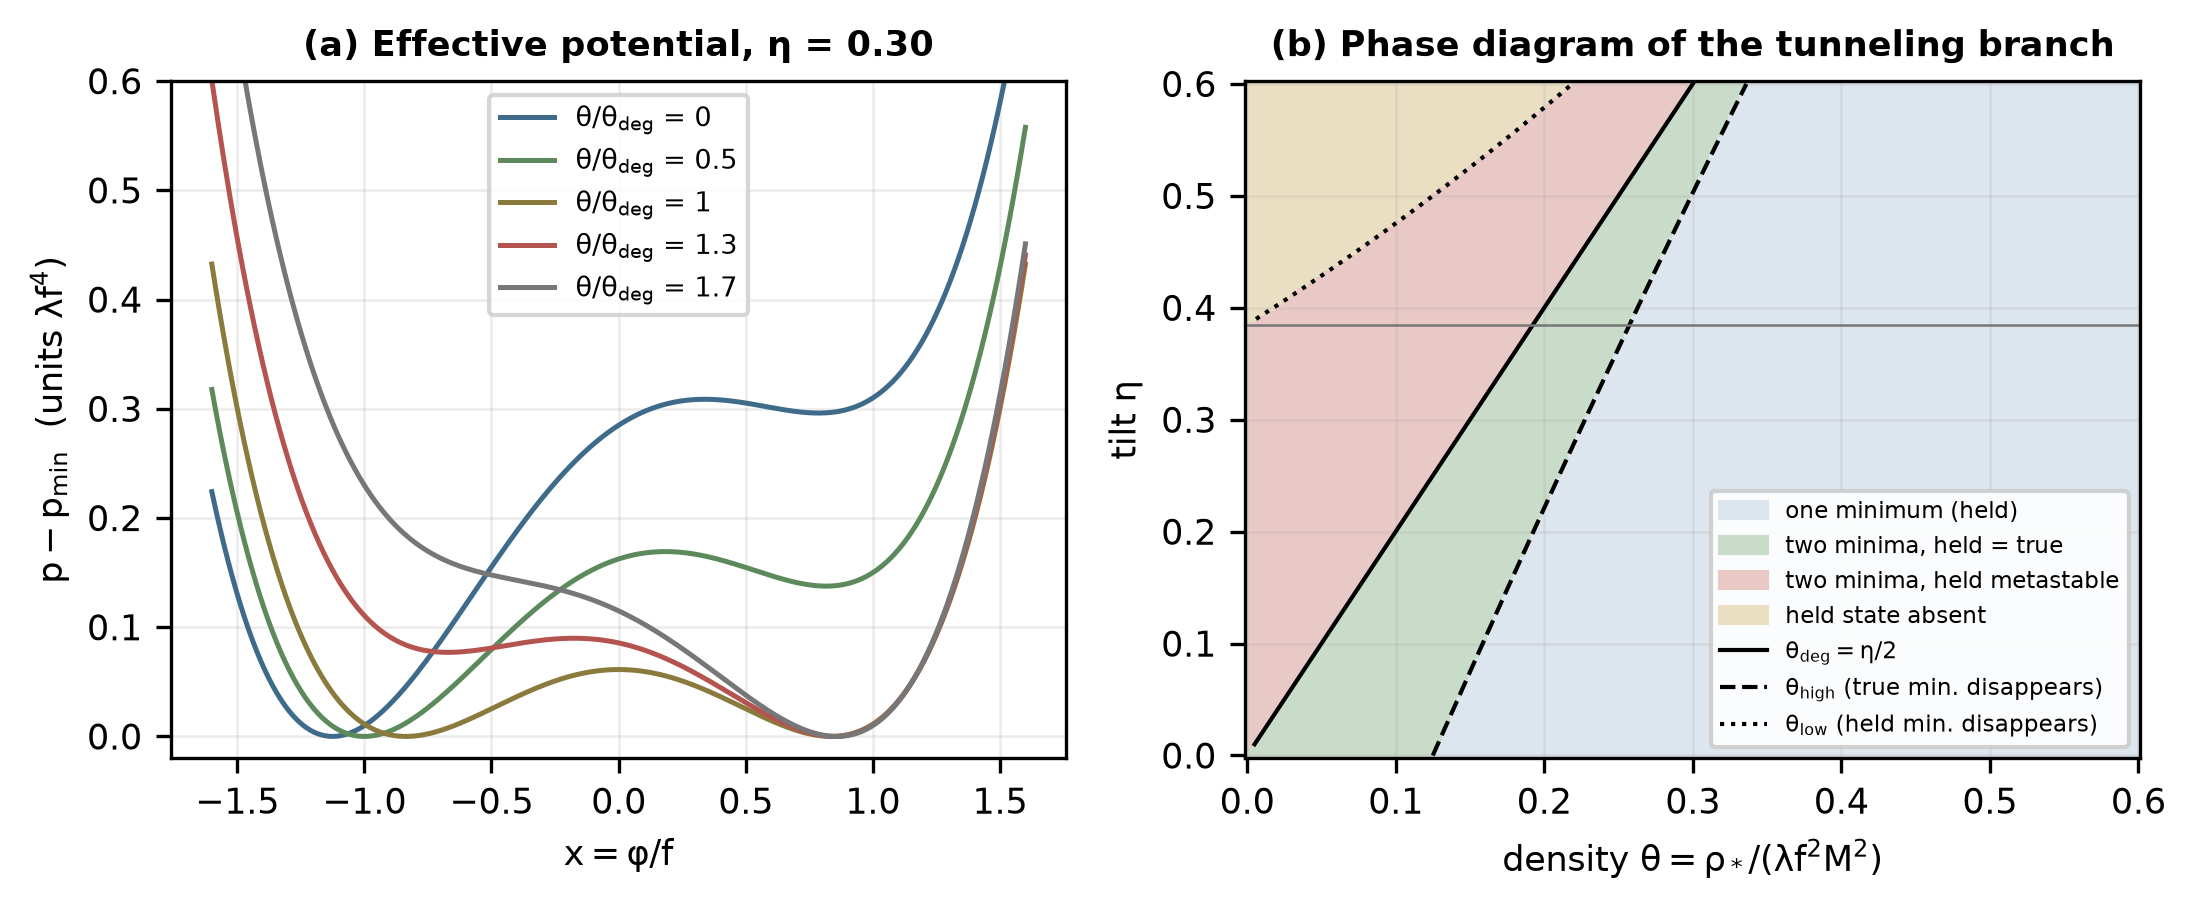
\includegraphics[width=1.00\textwidth]{../figures/fig1_vacuum_landscape.png}\caption{(a) Effective potential at five densities ($\eta=0.30$): dilution turns the matter-held minimum near $x=1$ from the true into the false vacuum at $\theta_{\rm deg}=\eta/2$. (b) Phase diagram: number of minima and which is lower, with the degeneracy line and the lines where a minimum disappears; the gray line marks $\eta_c$.}\end{figure}
\section{When does the field feel a smooth dark-matter density?}
\subsection{The scales of the problem}
The effective potential $V_0+\rho_*A$ is a mean-field statement. The field responds to sources within its Compton length $m_\varphi^{-1}$, with $m_\varphi^2=\lambda f^2\,\partial_x^2p(x_h)$ at the held vacuum, and on the time scale $m_\varphi^{-1}$; the bounce itself has a radius of a few Compton lengths. Normalized to the observed dark energy (Section 4.3), $m_\varphi=3.01$ meV at the trigger and 3.18 meV today, a Compton length of 0.066 mm (granularity.py). The mean dark-matter energy density at the trigger is 3.74 meV$^4$, so

\begin{equation}
\frac{\rho_{\rm dm}}{m_\varphi^4}=0.046\ \ (\text{trigger}),\qquad 0.094\ \ (\text{today})
\end{equation}
Less than one field-mass worth of dark matter lies in a Compton volume. Whether the source is nevertheless smooth depends on what the dark matter is, and three cases must be distinguished (Table 1, Fig. 2a).

\subsection{Particle dark matter}
If the dark matter consists of particles whose occupation of phase space is small, the source of the field is a set of points. The mean field applies only if many of them lie inside a Compton volume, $n_{\rm dm}\gg m_\varphi^3$, which requires $m_{\rm dm}\ll\rho_{\rm dm}/m_\varphi^3=0.14$ meV. A particle description, on the other hand, needs an occupation per de Broglie cell below one, $m_{\rm dm}\gg(\rho_{\rm dm}/v^3)^{1/4}=247$ meV for a velocity dispersion $v=10^{-3}$. The two conditions exclude each other, and fermions lighter than a few hundred eV are excluded in any case by phase-space bounds [21]. For thermal relics the mismatch is large: the mean separation of 1 MeV particles is 1940 times the Compton length and that of 1 GeV particles 19395 times. Each particle is a screened point source around which the field is pinned within a Compton length, as for the thin-shell objects of chameleon screening [4]; between them the field sees zero density. If so, the held vacuum decays in the space between the particles at the zero-density rate, $\ln(\Gamma/H^4)=88$ in the baseline, and the expected number of bubbles in our past light cone is $e^{86}$. Under this local mean-field criterion particle dark matter does not provide a smooth source on the response scale of the field; Section 3.5 tests the consequence with a spatially resolved calculation. The bound is least severe where it does not matter: in haloes the density is highest, but there the held vacuum is the true vacuum and nothing decays (Section 4.4); in the voids, where the decay must begin, the density is lower than the mean and the bound is stronger.

\subsection{Wave dark matter}
A bosonic dark matter with a large occupation number is a classical field oscillating at its mass [22], and its coupling through $A^2(\varphi)g_{\mu\nu}$ gives the field a source proportional to the instantaneous trace of its stress-energy. Two regimes follow. If the dark matter is lighter than the field, $m_{\rm dm}\ll m_\varphi$, the field follows the oscillation; the source passes through zero twice per period, and tunneling, which takes a time of order $m_\varphi^{-1}$, proceeds in those intervals at the zero-density rate, with the same consequence as for particles. If it is heavier, $m_{\rm dm}\gg m_\varphi$, the source oscillates faster than the field can respond, and the field feels its time average, which for a nonrelativistic field is $\rho_*A(\varphi)$. The source is also smooth in space, because the field is coherent over its de Broglie length $1/(m_{\rm dm}v)$, which exceeds the Compton length for $m_{\rm dm}\ll m_\varphi/v=3.0$ eV. Together with classicality, the mean field of Section 2 applies for

\begin{equation}
m_\varphi=3.0\ {\rm meV}\ \ll\ m_{\rm dm}\ \ll\ \left(\frac{\rho_{\rm dm}}{v^3}\right)^{1/4}=247\ {\rm meV}
\end{equation}
at the trigger, a window of approximately two decades, which widens slightly in the emptier, colder voids where the trigger begins. Dark matter in this mass range is a nonthermal condensate, produced for instance by misalignment [23], and behaves as cold dark matter on all scales that have been observed [22]. The trigger of this paper therefore specifies the dark matter: a classical bosonic field of meV to sub-eV mass. Everything that follows assumes it.

The averaging can be made explicit. The conformal coupling gives the field equation the source $-(A'/A)\,T_{\rm dm}$, with $T_{\rm dm}$ the trace of the dark-matter stress-energy. For a homogeneous nonrelativistic field oscillating at $m_{\rm dm}$ the pressure is $p=-\rho\cos(2m_{\rm dm}t)$, so $T_{\rm dm}=-\rho\,[1+3\cos(2m_{\rm dm}t)]$: the average is the $-\rho$ of a pressureless fluid, and the oscillating part drives the field at the frequency $2m_{\rm dm}$. The response of a field of mass $m_\varphi$ to that drive is smaller than its response to a static source by $m_\varphi^2/(4m_{\rm dm}^2-m_\varphi^2)$, so the residual modulation of the density the field feels is $3(m_\varphi/2m_{\rm dm})^2$, below 1\% for $m_{\rm dm}\ge10m_\varphi$ and growing to order one as $m_{\rm dm}$ approaches $m_\varphi$, where the two regimes meet. Fluctuations of the dark-matter density on scales between the de Broglie length and the size of a void are part of the local density of Section 4.4, not of its granularity. Section 5 tests the averaging dynamically, with a wall running through wave dark matter.

\begin{table}[htbp]\centering\small
\caption{Coupled dark matter and the density the field feels at the trigger ($m_\varphi=3.0$ meV, $\rho_{\rm dm}=3.74$ meV$^4$, $v=10^{-3}$).}
\begin{tabular}{>{\raggedright\arraybackslash}p{0.204\dimexpr\textwidth-8\tabcolsep\relax}>{\raggedright\arraybackslash}p{0.395\dimexpr\textwidth-8\tabcolsep\relax}>{\raggedright\arraybackslash}p{0.256\dimexpr\textwidth-8\tabcolsep\relax}>{\raggedright\arraybackslash}p{0.145\dimexpr\textwidth-8\tabcolsep\relax}}
\toprule
Dark matter & Condition & What the field feels & Trigger \\ \midrule
particle, any mass & point sources; $n\gg m_\varphi^3$ needs $m<0.14$ meV, particle regime needs $m>247$ meV & zero-density rate between particles & excluded \\
fermion, light & phase-space (Tremaine--Gunn) bound & -- & excluded \\
wave, $m_{\rm dm}\ll m_\varphi$ & field follows the oscillation & zero-density rate at the nodes & excluded \\
wave, $m_\varphi\ll m_{\rm dm}\ll247$ meV & time average, coherent over the de Broglie length & mean field $\rho_*A(\varphi)$, local density & viable \\
\bottomrule
\end{tabular}
\end{table}
\subsection{Why the bound is generic}
The smallness of $\rho_{\rm dm}/m_\varphi^4$ is not a property of the baseline. With $\lambda f^4=(1+q)V_f/\Delta\tilde V_0$ fixed by the observed dark energy and $m_\varphi^4=\lambda^2f^4\,(\partial_x^2p)^2$,

\begin{equation}
\frac{\rho_{\rm dm}}{m_\varphi^4}=\frac{\rho_{\rm dm}}{V_f}\,\frac{\Delta\tilde V_0}{1+q}\,\frac{1}{\lambda\,(\partial_x^2p)^2},\qquad \lambda=\frac{b(\eta,\theta)}{B}
\end{equation}
The first factor is of order one because the dark matter and the dark energy have comparable densities, which is what makes a dilution trigger possible in the first place; and $\lambda$ is fixed by the requirement that the transition happen within a Hubble time, $B\approx287$. Over all 153 combinations of tilt, density and $q$ in the bounce tables the ratio stays below 2.5. Toward $\eta_c$, where the held minimum becomes shallow, both $\lambda$ and $\partial_x^2p$ fall and the ratio grows, but only at vanishing density: it reaches 745 at $\eta=0.384$ and $\theta=0$, and stays below 5.2 once $\theta\ge0.1\,\theta_{\rm deg}$, the densities at which the decay is triggered. Particle dark matter would need a ratio above $1/v\approx10^3$. The coincidence of the dark-matter and dark-energy densities, which motivates a dilution trigger, is thus what makes particle dark matter fail the criterion.

\begin{figure}[htbp]\centering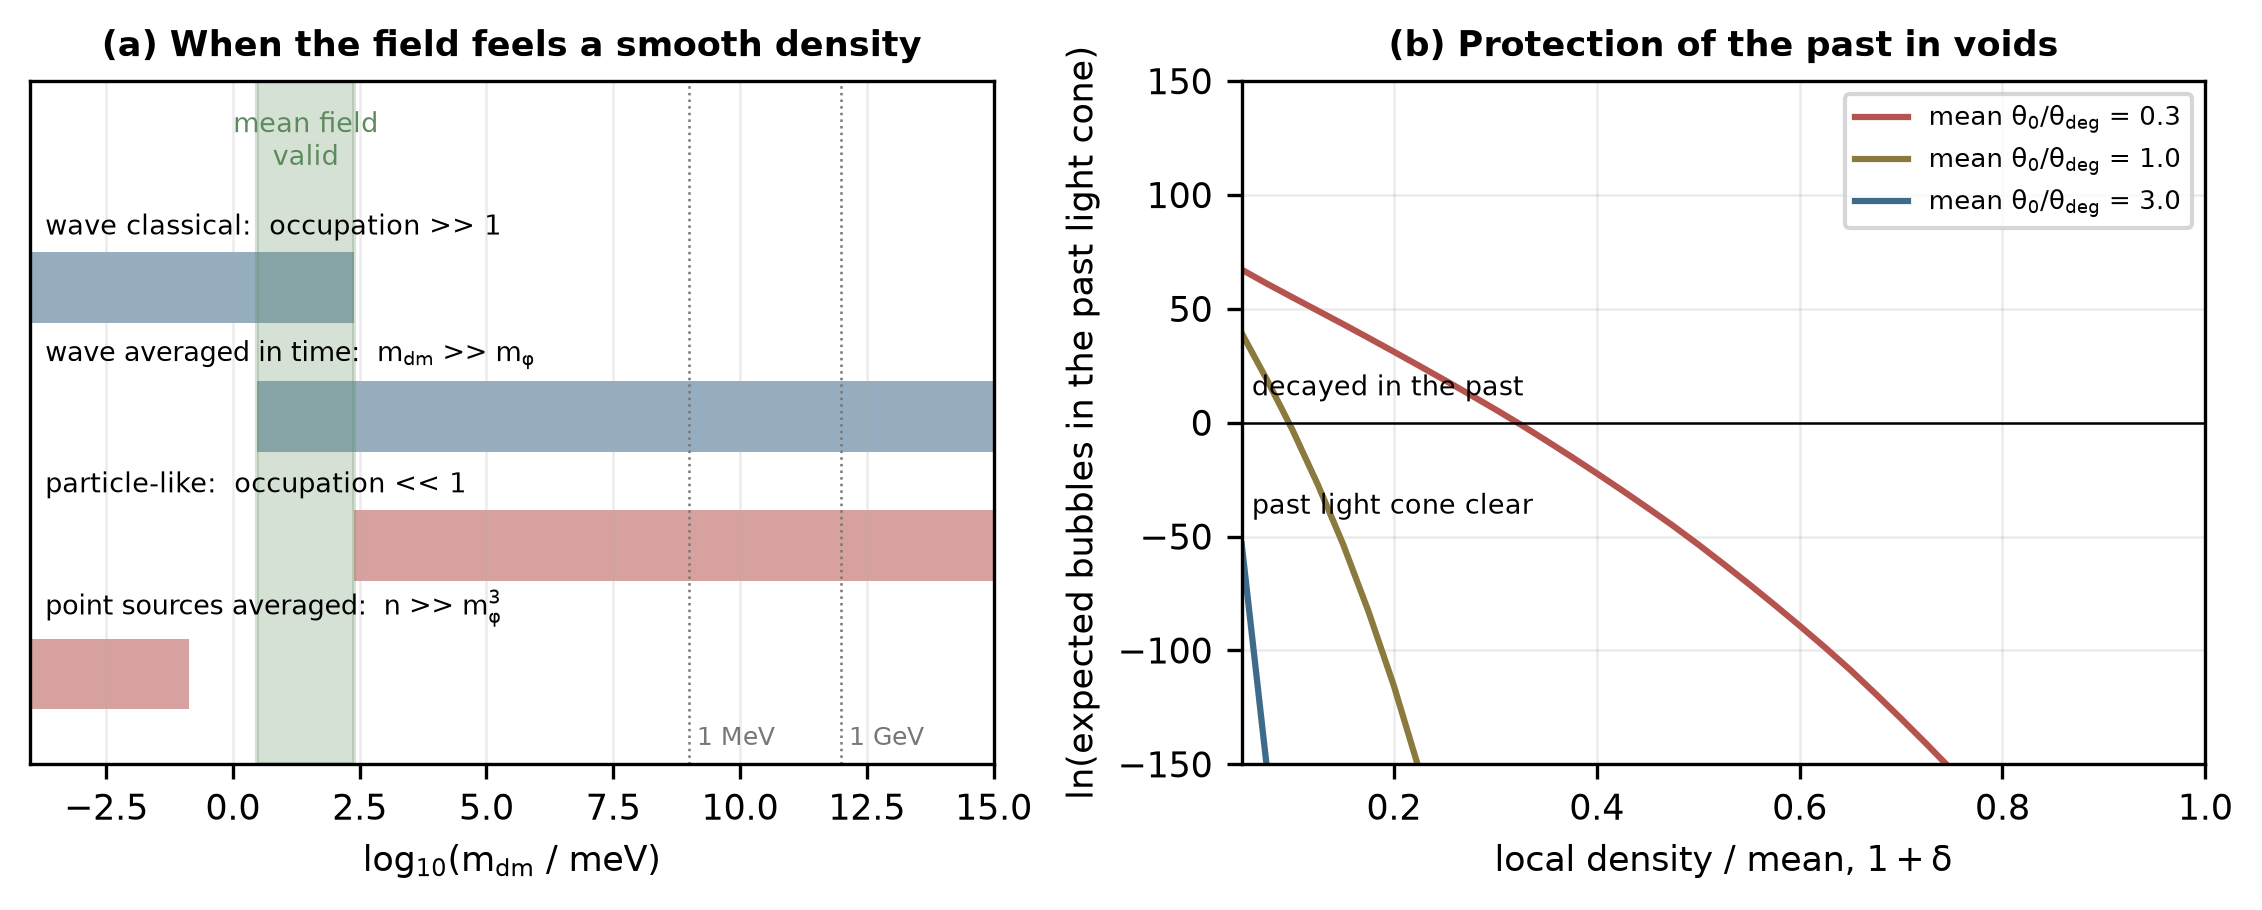
\includegraphics[width=1.00\textwidth]{../figures/fig2_granularity.png}\caption{(a) Conditions for the field to feel a smooth dark-matter density at the trigger: particle dark matter (red) needs two incompatible conditions; wave dark matter (blue) is averaged where it is heavier than the field and still classical (green band). (b) Expected number of bubbles in the past light cone of a region whose density is a fraction $1+\delta$ of the mean, for three mean couplings today ($\eta=0.30$, $q=1$, $B_0=200$): the emptiest regions decide whether the past is protected.}\end{figure}
\subsection{Spatially resolved tests}
Two calculations replace the criterion by a resolved treatment (granular\_field.py). The first solves the static field equation $\nabla^2x=\partial_xp_0(x)+\theta_s(\mathbf r)(x-1)$ in a spherical Wigner--Seitz cell around one source, with the source spread over a sphere small compared with the cell and normalized so that the cell average of $\theta_s$ is the mean coupling at the trigger. For cells smaller than the Compton length the field is uniform at the mean-field minimum; for a cell radius $R_c=6.5/m_\varphi$ the field lies within 1\% of the zero-density vacuum in 96\% of the cell volume, and in 99.8\% for $R_c=20/m_\varphi$ (Fig. 3a); the fraction changes by less than 1\% when the radius of the source is varied tenfold. The crossover lies at a cell radius of a few Compton lengths.

The second computes the decay rate in a granular background. A static source at distance $r_p$ from the center of the zero-density bounce adds to the Euclidean action, at first order in its coupling $q$ (the coupling carried by one particle), $\Delta B=(q/\lambda)I(r_p)$ with $I(r_p)=\int d\tau\,\frac12[(x_b-1)^2-(x_h-1)^2]$ along its worldline. For sources placed at random with number density $n$,

\begin{equation}
\frac{\Gamma}{\Gamma_0}=\Big\langle e^{-\sum_i\Delta B_i}\Big\rangle=\exp\!\Big[-n\int d^3r\,\big(1-e^{-qI(r)/\lambda}\big)\Big]
\end{equation}
For many weak sources this reduces to the first-order mean-field suppression $\exp(-\theta\,\partial_\theta b/\lambda)$, and the derivative obtained in this way agrees with the numerical derivative of the bounce action to 0.23\%. For few strong sources it reduces to $\Gamma_0$ times the probability that the bounce region contains no source. At the trigger density the suppression falls to half of its mean-field value for point sources of mass 3 meV, and to fractions $7\times10^{-8}$ and $8\times10^{-11}$ of it for 1 MeV and 1 GeV particles (Fig. 3b): with particle dark matter the vacuum decays at its zero-density rate. The first-order treatment overstates the suppression from a strong source, because the field near the source saturates and the bounce can deform around it, so for heavy particles the true rate is at least as close to $\Gamma_0$. The calculation treats the particles as static over the time of the bounce, which holds for $v\ll1$, and does not construct a fully four-dimensional inhomogeneous bounce. Within these approximations it confirms the criterion: conventional particle dark matter does not provide a smooth source on the response scale of the field, and a density-triggered decay of a vacuum at this scale requires wave dark matter.

\begin{figure}[htbp]\centering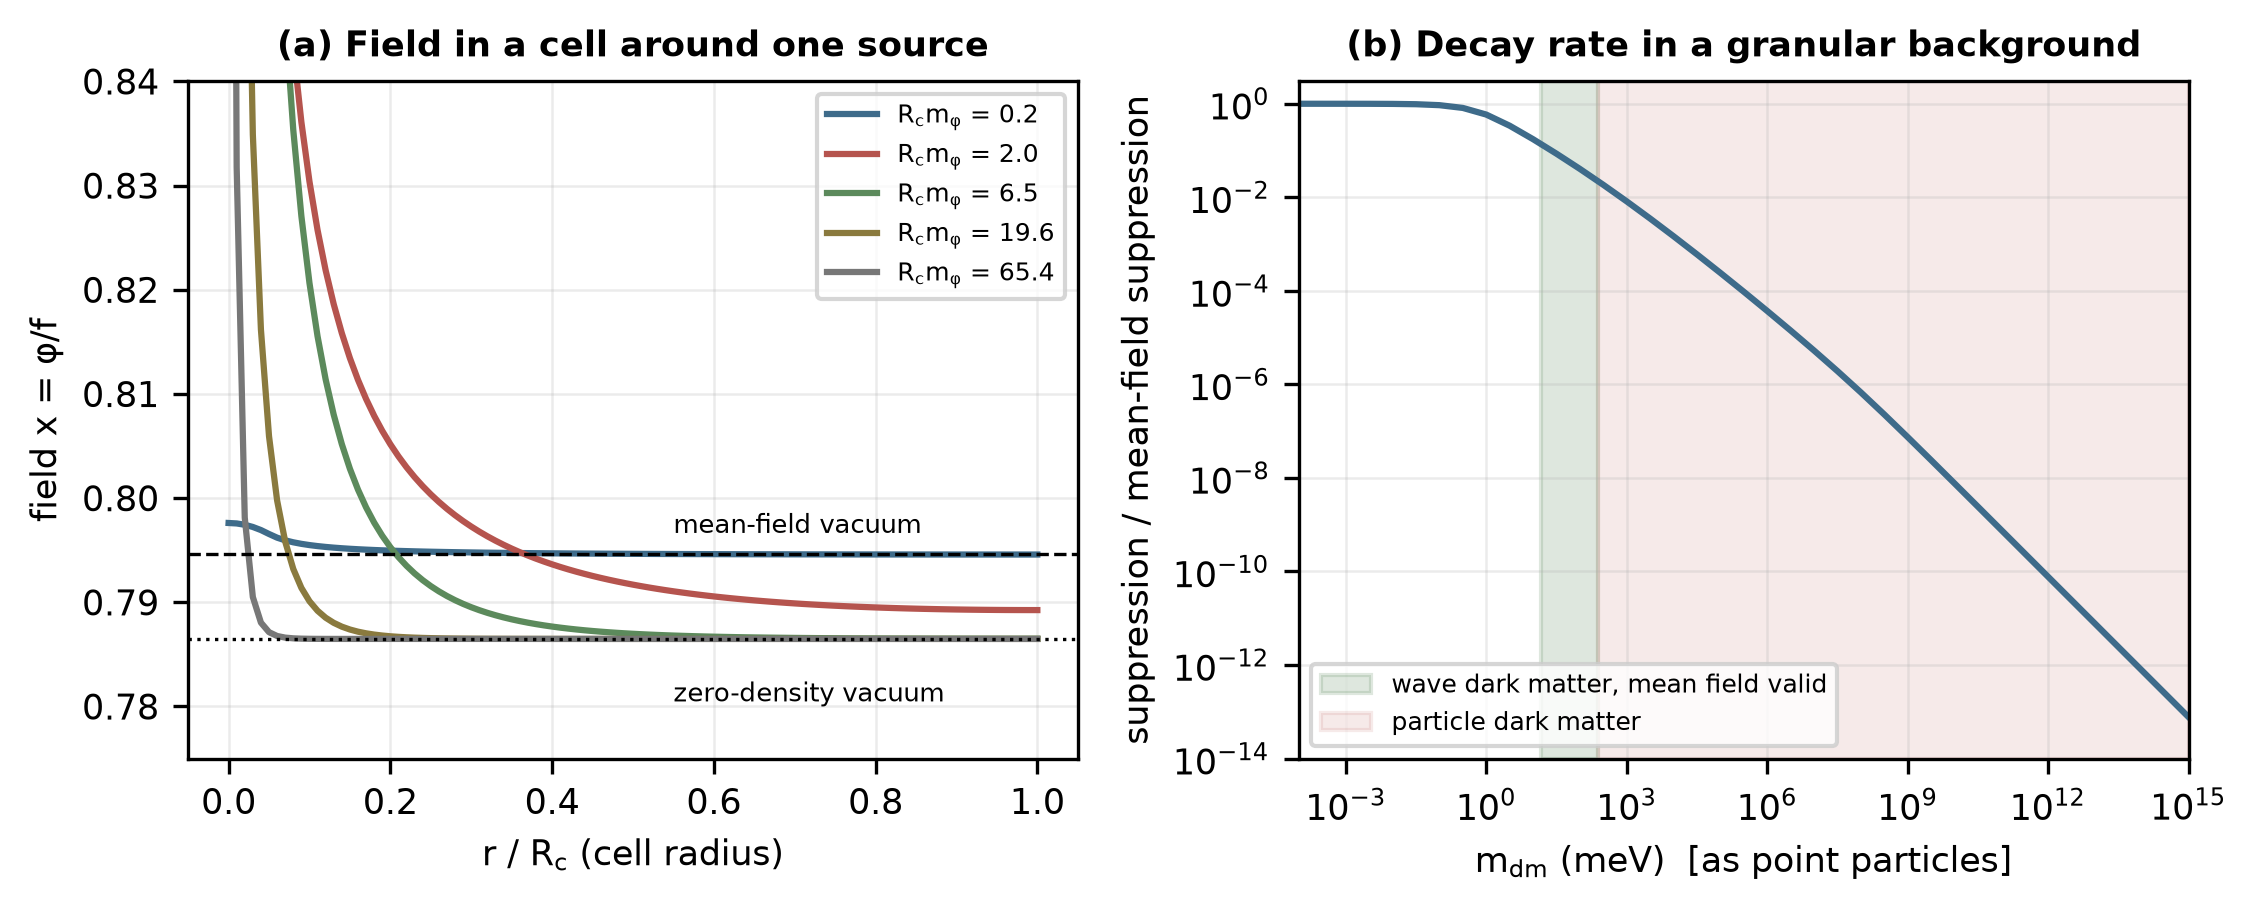
\includegraphics[width=1.00\textwidth]{../figures/fig3_resolved_granularity.png}\caption{(a) Static field in a Wigner--Seitz cell around one dark-matter source at the trigger coupling, for cells from 0.2 to 65 Compton lengths: small cells reproduce the mean-field vacuum, large cells the zero-density vacuum away from the source. (b) Suppression of the decay rate by randomly placed point sources, relative to the first-order mean-field suppression, against the particle mass at the trigger density; shaded, the wave-dark-matter window of Section 3.3 and the particle regime.}\end{figure}
\section{Density-dependent bubble nucleation}
\subsection{The bounce and its action}
Where the mean field applies, the O(4)-symmetric bounce solves, in units of $f$ for the field and $(\sqrt\lambda f)^{-1}$ for lengths,

\begin{equation}\begin{gathered}
x''+\frac{3}{r}x'=\partial_xp(x;\eta,\theta),\qquad x'(0)=0,\\
x(\infty)=x_h,\qquad b(\eta,\theta)=2\pi^2\int_0^\infty r^3\left[\frac{x'^2}{2}+p(x)-p(x_h)\right]dr
\end{gathered}\end{equation}
and the action is $B=b/\lambda$ [1, 2]. Gravity enters only through $g=f^2/M_{\rm Pl}^2$, of order $10^{-60}$ at the dark-energy scale, so the flat-space bounce is exact for all practical purposes [3, 24]; Section 6 confirms that the wall's own gravity is negligible. The bounce is found by overshoot and undershoot on the central value with an eighth-order Runge--Kutta integrator; where the central value lies within $10^{-5}$ of the true minimum (the thin-wall regime) shooting becomes exponentially sensitive and collocation on the boundary-value problem is used instead (vacuum\_wall.py). At $\theta=0$ the actions reproduce an independent table to $2\times10^{-12}$, and where both methods apply they agree to the tolerance of the collocation.

\subsection{The wall}
The interface follows from the field equations rather than being imposed. At the degeneracy density the static planar wall, $x''=\partial_xp$, has the first integral $z(x)=\int dx/\sqrt{2(p-p_{\rm min})}$, tension $\sigma=\int\sqrt{2(p-p_{\rm min})}\,dx=0.390\,\sqrt\lambda f^3$ and 10--90\% thickness $5.3/(\sqrt\lambda f)$ for $\eta=0.30$; the symmetric case $\eta=\theta=0$ reproduces $\sigma=2/3$ and $x=\tanh(z/2)$. Below the degeneracy density a static planar wall does not exist, since the energy difference accelerates it, and the wall is read from the bounce: its tension $\sigma_b=\int x'^2dr$ and its thickness change little with density, while the radius grows from $6.7$ to $13.6$ and the action from $b=441$ to $5250$ between $\theta=0$ and $0.6\,\theta_{\rm deg}$ (Table 2, Fig. 4a,b). The thin-wall action

\begin{equation}
B_{\rm tw}=\frac{27\pi^2\sigma^4}{2\,\Delta V^3},\qquad \sigma=\int_{x_t}^{x_h}\sqrt{2\,[p(x)-p_{\rm lin}(x)]}\,dx
\end{equation}
with $p_{\rm lin}$ the straight line through the two minima, which removes the energy difference from the tension, is recovered within 1\% from $0.6\,\theta_{\rm deg}$ upwards for $\eta=0.20$ and 0.30, and overestimates the thick-wall bounce near zero density ($b/B_{\rm tw}=0.86$ at $\theta=0$ for $\eta=0.30$). The density dependence of the action is therefore dominated by $\Delta V(\theta)$, which falls linearly to zero at $\theta_{\rm deg}$, while the tension is nearly constant.

\begin{table}[htbp]\centering\footnotesize\setlength{\tabcolsep}{3pt}
\caption{Bounce and wall against density ($\eta=0.30$, units $\lambda f^4$, $(\sqrt\lambda f)^{-1}$ and $\sqrt\lambda f^3$).}
\begin{tabular}{llllllll}
\toprule
$\theta/\theta_{\rm deg}$ & $\Delta V$ & $b$ & $b/B_{\rm tw}$ & $R_w$ & thickness & $\sigma_b$ & method \\ \midrule
0.00 & 0.296 & 441 & 0.86 & 6.7 & 5.58 & 0.484 & shooting \\
0.10 & 0.263 & 601 & 0.90 & 7.2 & 5.38 & 0.492 & shooting \\
0.20 & 0.230 & 836 & 0.93 & 7.8 & 5.24 & 0.495 & shooting \\
0.30 & 0.199 & 1201 & 0.96 & 8.6 & 5.15 & 0.493 & shooting \\
0.40 & 0.168 & 1809 & 0.98 & 9.7 & 5.09 & 0.487 & shooting \\
0.50 & 0.138 & 2921 & 0.99 & 11.3 & 5.06 & 0.478 & shooting \\
0.60 & 0.108 & 5250 & 1.00 & 13.6 & 5.05 & 0.466 & shooting \\
0.70 & 0.080 & 11256 & 1.01 & 17.1 & 5.07 & 0.454 & collocation \\
0.80 & 0.052 & 33678 & 1.01 & 25.0 & 5.10 & 0.435 & collocation \\
\bottomrule
\end{tabular}
\end{table}
\subsection{Physical scale, survival and the trigger}
We normalize to the observed universe: the false vacuum carries the observed dark-energy density $V_f$, the true vacuum $V_t=-qV_f$ with $q=1$, so that $\lambda f^4=(1+q)V_f/\Delta\tilde V_0$, and the action at zero density is $B_0=b(0)/\lambda=200$ for $\eta=0.30$. Then $f=2.97$ meV and the wall scale $1/\sqrt\lambda f$ is 0.045 mm. The rate per unit four-volume is $\Gamma=\mathcal A\,e^{-B(\theta)}$ with the one-loop prefactor estimated as $(B/2\pi)^2$ times the fourth power of the false-vacuum mass scale [2], and the relevant comparison is with the Hubble four-volume, $\Gamma/H^4$. The probability that no bubble has nucleated in the past light cone of a present observer is $\exp(-\int\Gamma\,dV_4)$; in the observed $\Lambda$CDM history the four-volume of the past light cone is $V_4=0.0591\,H_\Lambda^{-4}$, 445 times smaller than the Euclidean four-sphere often used as a shortcut, so that survival requires only $\Gamma/H_\Lambda^4\lesssim51$ for a constant rate [25, 26]. With the coupling the rate in the past was suppressed by the larger density, and the survival integral is evaluated with the density history $\theta=\theta_0(1+z)^3$. In the future the rate rises as the matter dilutes (Fig. 4c), and the transition completes, in the sense that bubbles percolate, once $\Gamma/H^4>9/4\pi$ [25]. The prefactor is the least certain input: a full one-loop determinant [27] could differ from the estimate by a factor comparable to $(B/2\pi)^2$ itself, $e^{7.6}$ at the trigger. Because the rate grows at $\beta=351\,H$ (Section 6), such a factor moves the completion by 0.02 Hubble times, and it moves the boundary of the region with a protected past by the same 7.6 units in $B_0$; the qualitative results do not depend on it.

Because the field responds to the local density (Section 3.3), these statements hold region by region, with $\theta_0$ the local value. For a region with $\theta_0=0.3\,\theta_{\rm deg}$, the baseline of this paper, the past light cone is clear and the transition completes at $a=1.37$, when $\theta=0.116\,\theta_{\rm deg}$ and $B=287$; the nucleated bubble has radius 0.33 mm, wall thickness 0.24 mm and tension 19 meV$^3$.

\subsection{The environment: voids first, haloes last}
The rate depends exponentially on the local density, so the emptiest regions decide both whether the past is protected and when the decay begins. The deepest cosmic voids have central densities of 10--20\% of the mean [28]. If a region with $1+\delta$ times the mean density is followed through the whole past light cone with that contrast (conservative, since voids were less empty in the past), the past light cone of a region at the mean density is clear for any mean coupling above $\theta_0=0.10\,\theta_{\rm deg}$, but a region at 20\% or 10\% of the mean requires $\theta_0\ge0.48$ or $0.97\,\theta_{\rm deg}$ on average (Fig. 2b; granularity.py). With the mean coupling of Section 4.3 taken as the mean rather than the void value, regions at 30\% of the mean or less would already have decayed. A protected past therefore requires a mean coupling today close to the degeneracy density, and the baseline of Section 4.3 is to be read as the local value in voids at 10\% of the mean, $\theta_0=3.0\,\theta_{\rm deg}$ on average.

With that mean, the held vacuum is still the true vacuum wherever $1+\delta>\theta_{\rm deg}/\bar\theta(a)$: at the trigger this is any region denser than 0.86 times the mean, and the threshold rises as $a^3$. A bubble nucleated in a void expands through all connected regions in which the held vacuum is metastable, and its wall stalls where the local density reaches the degeneracy value, because the driving pressure, proportional to $\Delta V_{\rm eff}$, vanishes there and changes sign beyond. The transition therefore advances from the voids into sheets and filaments as the universe expands, following the contour $\theta_{\rm loc}=\theta_{\rm deg}$, while virialized haloes, whose density does not dilute, keep the held vacuum indefinitely: a galactic halo at approximately two hundred times the mean density has $\theta\approx600\,\theta_{\rm deg}$, far above $\theta_{\rm high}=1.52\,\theta_{\rm deg}$, where only the held minimum exists. The dark energy measured inside galaxies is therefore unchanged by the transition, and the haloes become islands of the held vacuum bounded by walls whose tension energy is negligible ($9\times10^{-31}$ kg per square metre for the baseline tension). Separate voids are separated by such walls at the trigger and must each nucleate a bubble; since the rate grows at $\beta=351\,H$ (Section 6), a void of comoving radius 5--50 Mpc does so within 0.033--0.053 Hubble times of the global completion criterion.

The advance of the transition can be read off the threshold $1+\delta_*(a)=a^3\theta_{\rm deg}/\bar\theta_0$: 0.86 at the trigger, 2.7 at $a=2$, 9.0 at $a=3$ and 42 at $a=5$. Sheets and the outskirts of filaments, a few times denser than the mean, are swept within a Hubble time of the trigger; the cores of filaments, ten or more times the mean, only later; virialized structures never, because their density does not fall. Two features distinguish this from vacuum decay seeded by inhomogeneities elsewhere in the literature. Compact objects such as black holes catalyse the decay of a metastable vacuum by lowering the action in their vicinity [29, 30]; here the seed is the absence of matter, and the decay is suppressed, not catalysed, where matter has collapsed. And the wall does not need to overcome the denser regions: it stops where the held vacuum becomes the true vacuum, so that the outcome of the transition is a map of the cosmic density field at the time of the trigger.

The environment yields a quantitative relation. Because the field responds to the local density and the trigger depends on the coupling only through $\theta_0a^{-3}$, a region whose density is a fraction $1+\delta$ of the mean completes its transition at $a_{\rm tr}(\delta)=a_{\rm tr}(0)\,(1+\delta)^{1/3}$ while its contrast is frozen. For a mean coupling $\bar\theta_0=3\,\theta_{\rm deg}$ the computed values are $a_{\rm tr}=1.38$, 2.00, 2.96 and 3.73 for $1+\delta=0.1$, 0.3, 1 and 2 (viability\_extended.py), and a change of the one-loop prefactor by $(B/2\pi)^2$ moves them by at most 2\%. The order of the transition across the cosmic web, voids first and in the order of their emptiness, is a prediction of the mechanism. It is not observable today, because a protected past means that no transition has happened inside our past light cone; what is observable now is listed in Section 10.

\begin{figure}[htbp]\centering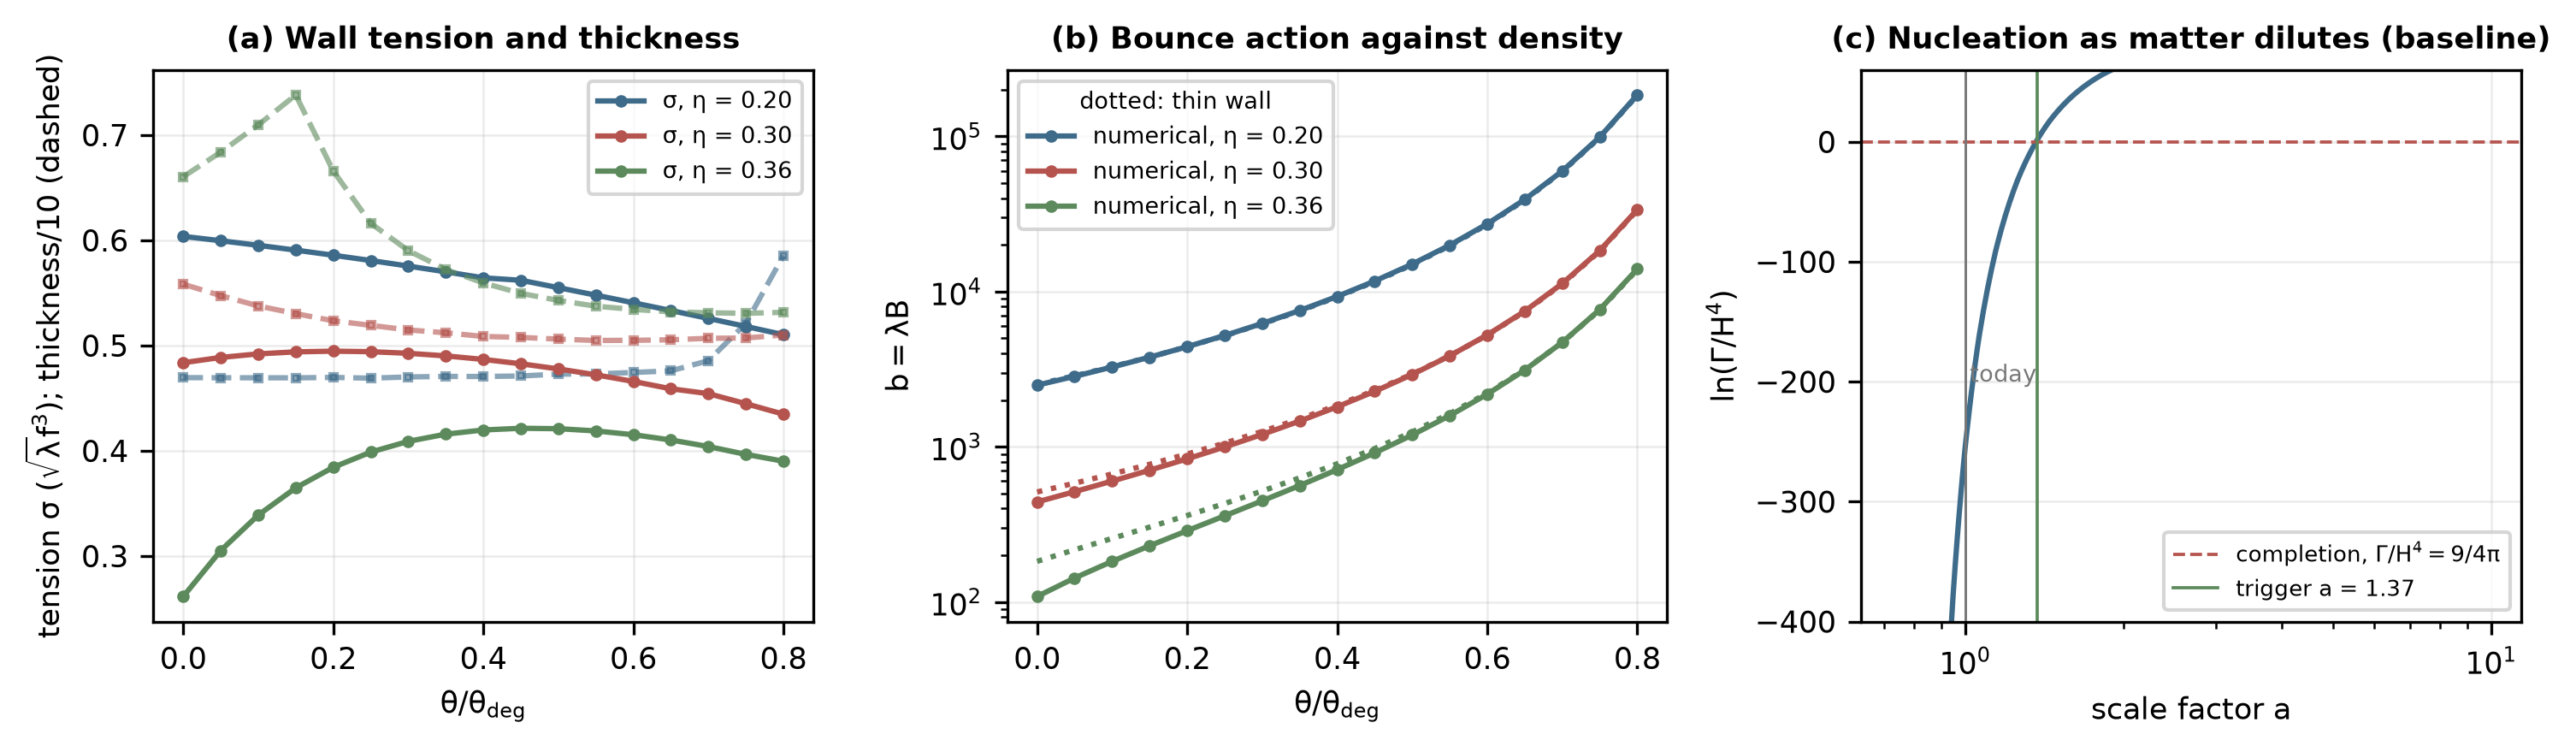
\includegraphics[width=1.00\textwidth]{../figures/fig3_interface_properties.png}\caption{(a) Wall tension (solid) and thickness/10 (dashed) of the O(4) bounce against density for three tilts. (b) Bounce action $b=\lambda B$, numerical (points) and thin-wall (dotted). (c) $\ln(\Gamma/H^4)$ along the dilution history of a region with $\theta_0=0.3\,\theta_{\rm deg}$, with the completion threshold and the trigger.}\end{figure}
\section{Interface tension and field transmission}
A wall makes the mass of every field coupled to $\varphi$ depend on position. For a test scalar with $\mathcal L_{\rm int}=-\frac12g^2\varphi^2\psi^2$, $m_\psi^2(z)=m_0^2+g^2f^2x(z)^2$, and the modes of the planar wall in its rest frame obey

\begin{equation}
\left[-\frac{d^2}{dz^2}+m_\psi^2(z)\right]u=(\omega^2-k_\parallel^2)\,u,\qquad T=\frac{k_+}{k_-}\frac{1}{|A|^2},\qquad R=\left|\frac{B}{A}\right|^2
\end{equation}
with a transmitted wave $e^{ik_+z}$ on the false-vacuum side, integrated back across the wall and decomposed into $Ae^{ik_-z}+Be^{-ik_-z}$ on the true-vacuum side (interface\_transport.py). The same equation describes the wave dark matter of Section 3.3, whose mass changes by the factor $A(x_t)/A(x_h)$ across the wall. The solver is validated on the symmetric kink, for which $m^2=g^2f^2-g^2f^2\,{\rm sech}^2(z/2)$ is a Poeschl--Teller well with the exact transmission $T=\sinh^2(2\pi q)/[\sinh^2(2\pi q)+\cos^2(\frac\pi2\sqrt{1+16g^2/\lambda})]$; the numerical values agree with it to $2\times10^{-6}$, including the reflectionless coupling $g^2/\lambda=1/2$, and $T+R=1$ holds to $2\times10^{-10}$ (Fig. 5b).

Through the wall at the trigger the interior is heavier for every coupling ($m_{\rm in}/m_{\rm out}=1.32$, since $|x_t|>|x_h|$). Modes below the interior threshold are reflected, and above it $T$ exceeds 0.5 within $0.1\sqrt\lambda f$ of the threshold for every coupling tested (Fig. 5a). The interface is selective, but kinematically: it filters by mass, as any step does, with little additional reflection from its shape. Photons, neutrinos and baryons do not couple to $\varphi$ and cross unchanged. A thermal bath of test scalars exerts on a static wall a reflected momentum flux that is at most $7\times10^{-5}$ of the driving pressure at temperatures up to the wall scale, and in the ultrarelativistic limit at most $\Delta m^2T^2/24$ per degree of freedom [15]; at the CMB temperature of the trigger epoch this is below $5\times10^{-4}$ of the driving pressure.

For the coupled dark matter the mass ratio across the wall is $A(x_t)/A(x_h)=2.72$, far larger than its kinetic energy, so a slow wall would reflect all of it, as at the filtering transitions of [14]. The wall is not slow. Its driving pressure exceeds the largest pressure the dark matter can exert, $\rho_*\Delta A$ (the Boedeker--Moore limit for quanta that are transmitted at high Lorentz factor [15]), by a factor 8, so it runs away; dark matter at rest crosses once the wall's Lorentz factor exceeds $A(x_t)/A(x_h)$, which happens within 0.89 mm of the nucleation point. The fraction of the dark matter swept by the wall before it becomes transparent is $(\gamma_{\rm th}R_0/R_{\rm coll})^3=2\times10^{-88}$. The interface is therefore transparent to the dark matter for all practical purposes, and the transitioned region inherits the dark matter of its surroundings with the heavier mass of the true vacuum.

For wave dark matter the crossing was simulated directly (wave\_wall\_1d.py). A planar wall, started at rest as a kink, accelerates through a homogeneous oscillating dark-matter field whose mass is $mA(x)$, with the full backreaction of the dark matter on the scalar and nothing prescribed about the crossing (Fig. 6). The wall follows hyperbolic motion, and a fit of it gives the Lorentz factor; at the end of the run this is 7.7\% and 7.7\% below that of a run with the static mean-field term for $m_{\rm dm}=10m_\varphi$ and $3m_\varphi$, a difference that changes by 0.3\% when the grid spacing is doubled, while the wall position changes by 0.3\%. The energy given to the dark matter per unit length swept is 4.07 times its initial density (4.08 for $3m_\varphi$), close to the sudden-crossing value $(1+r^2)/2=4.19$, with $r=A(x_t)/A(x_h)=2.72$, and well above the adiabatic value $r$: once the wall is relativistic the crossing is sudden, and the field keeps its amplitude and velocity rather than its number of quanta. The dark matter is not left at rest. Quanta that cross a relativistic wall into the heavier vacuum leave it with momentum $m(r^2-1)/2$ in the frame of the background and velocity $(r^2-1)/(r^2+1)=0.76$; the simulated mean velocity of the dark matter behind the wall is 0.75, and the dark matter forms a shell that trails the wall with its energy density raised by $1/(1-v)$ (16 against 17.5 predicted). The energy taken from the wall is 0.24 of its driving pressure, so the wall still runs away. In the transitioned region the dark matter carries 54\% more quanta than the adiabatic estimate and moves outward until the shells of neighbouring bubbles collide, after which its momentum redshifts away.

\begin{figure}[htbp]\centering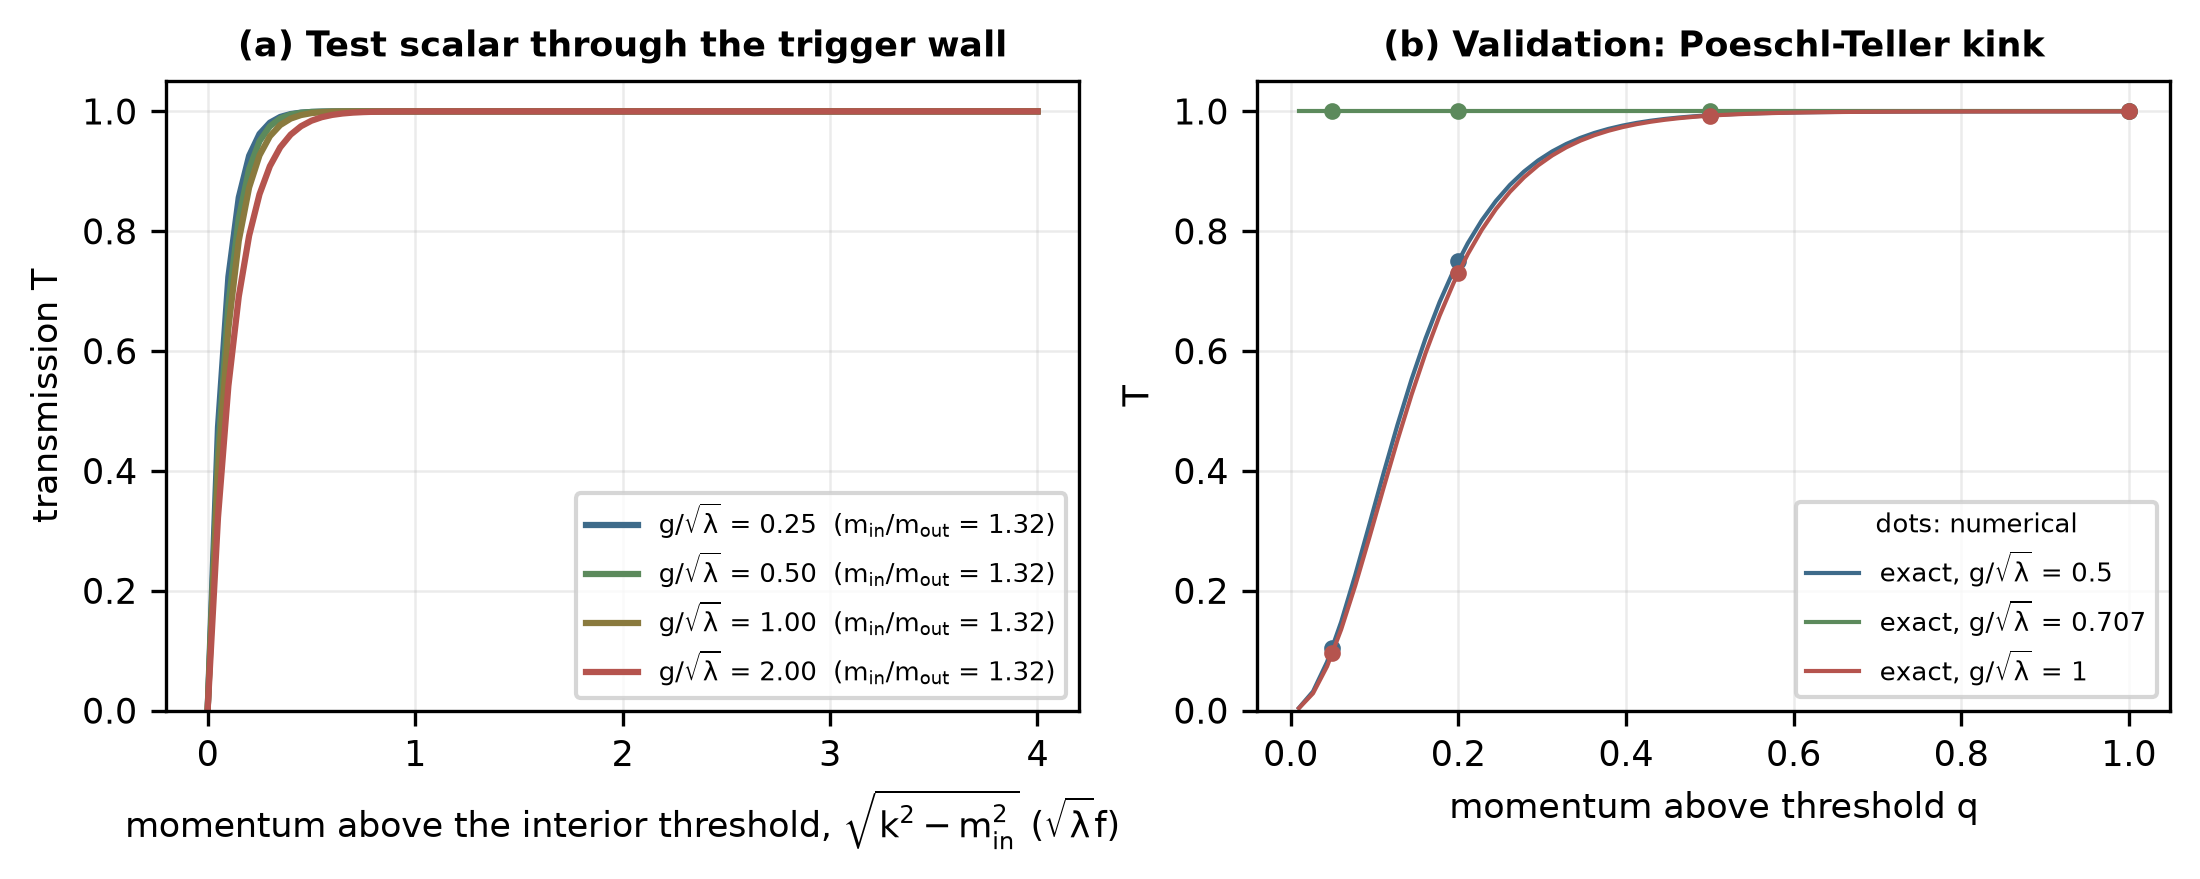
\includegraphics[width=1.00\textwidth]{../figures/fig4_selective_transmission.png}\caption{(a) Transmission of a test scalar through the wall at the trigger against momentum above the interior threshold, for four couplings. (b) Validation on the symmetric kink: numerical transmission (dots) against the exact Poeschl--Teller result (lines), including the reflectionless coupling $g^2/\lambda=1/2$.}\end{figure}
\begin{figure}[htbp]\centering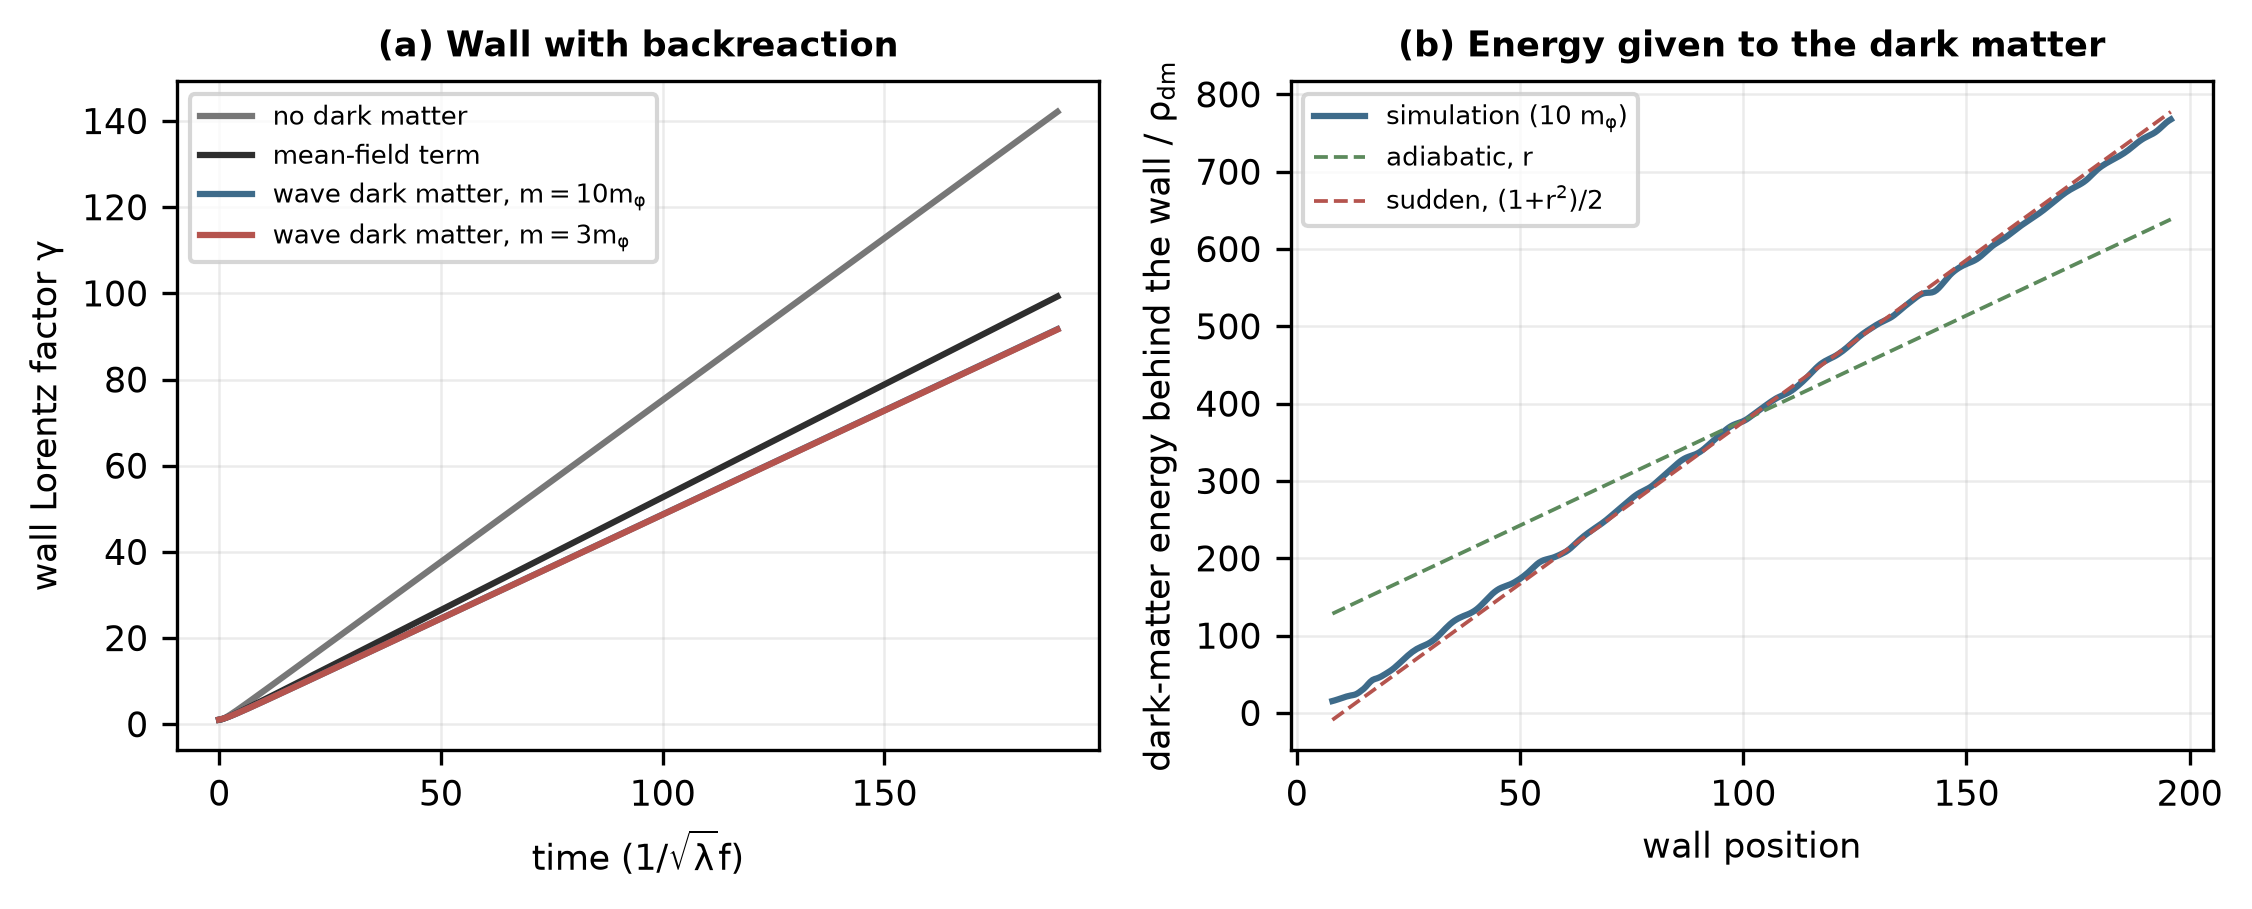
\includegraphics[width=1.00\textwidth]{../figures/fig6_wave_wall.png}\caption{A planar wall running through wave dark matter (1+1 dimensions, backreaction included). (a) Lorentz factor of the wall without dark matter, with the static mean-field term, and with wave dark matter of mass $10m_\varphi$ and $3m_\varphi$. (b) Dark-matter energy behind the wall against the wall position, with the adiabatic and sudden slopes.}\end{figure}
\section{Gravitational wall and collision dynamics}
For a thin wall of tension $\sigma$ and areal radius $R$ between an interior of density $\rho_-$ and an exterior of density $\rho_+$, the Israel junction condition can be written with the Misner--Sharp mass on each side [31, 17]:

\begin{equation}
\Gamma_--\Gamma_+=\frac{\sigma R}{2M_{\rm Pl}^2},\qquad \Gamma_\pm=\sqrt{1+\dot R^2-\frac{\rho_\pm R^2}{3M_{\rm Pl}^2}}\ \Rightarrow\ \Gamma_-=\frac{(\rho_+-\rho_-)R}{3\sigma}+\frac{\sigma R}{4M_{\rm Pl}^2}
\end{equation}
(bubble\_gravity.py). From $R_0=3\sigma/\Delta V$ (0.26 mm) to the Hubble radius the wall follows the flat-space runaway $\Gamma=R/R_0$ to round-off and reaches $\Gamma=$$5.9\times10^{29}$; its self-gravity, $\sigma R/2\Gamma$, is $2\times10^{-60}$; and the Misner--Sharp mass it carries equals the vacuum-energy deficit of the region it encloses (Fig. 7a). The released vacuum energy is therefore carried by the wall, not deposited in the interior, until walls collide or stall at the boundary of a denser region.

The completion of the transition in a connected region is computed from its rate history (bubble\_handoff.py): the false-vacuum fraction $f=e^{-I}$, $I=\frac{4\pi}{3}\int\Gamma a^3r^3dt$ with $r$ the comoving radius of a bubble nucleated at $t$ [25, 26], falls to one half at $a=1.462$ and to 1\% at $a=1.473$ (Fig. 8a). The rate grows at $\beta=d\ln\Gamma/dt=351\,H$, so the transition is completed in 0.019 Hubble times and the bubbles collide at a mean radius $R_{\rm coll}=(8\pi)^{1/3}/\beta=0.0084/H$, comparable to the size of large voids. At collision the walls have Lorentz factors of order $5\times10^{27}$.

The junction treatment omits several effects, which are bounded instead (Table 3). The Lorentz-contracted thickness of the wall is $4\times10^{-56}$ of its radius, so the thin-wall description is excellent once the wall has grown. The pressure of the dark matter is at most 0.13 of the drive. A dark gauge boson acquiring mass from $\varphi$ would add a pressure that grows with the Lorentz factor [16] and stop the runaway; for couplings $g\le1$ and any bath colder than 1 meV the terminal Lorentz factor is at least 1574, still above the threshold 2.7 at which the dark matter crosses, so the transparency of Section 5 is unchanged. Gravitational waves from the collisions carry at most a fraction $\sim8\times10^{-7}$ of the wall energy, suppressed by $(H/\beta)^2$, and since $R_{\rm coll}H\approx0.008$ no region of Hubble size is overdense enough to form black holes.

None of these signals is observable today. The trigger lies in the future, at $a\approx1.4$ for the baseline, and a protected past means precisely that no bubble has nucleated within our past light cone; the imprints of bubble collisions on the microwave background that have been studied for transitions in the early universe [12, 13] therefore do not arise. What is observable now is indirect: the dark energy is exactly $w=-1$ while the vacuum is held, and the dark matter must be of the kind specified in Section 3.

\begin{table}[htbp]\centering\small
\caption{Approximations of the wall dynamics and of the hand-off to the enclosed region, and their bounds (bubble\_handoff.py, granularity.py).}
\begin{tabular}{>{\raggedright\arraybackslash}p{0.315\dimexpr\textwidth-6\tabcolsep\relax}>{\raggedright\arraybackslash}p{0.484\dimexpr\textwidth-6\tabcolsep\relax}>{\raggedright\arraybackslash}p{0.202\dimexpr\textwidth-6\tabcolsep\relax}}
\toprule
Effect & Bound or result & Consequence \\ \midrule
mean-field source & wave dark matter, 3 meV $\ll m_{\rm dm}\ll$ 247 meV & required (Section 3) \\
completion of the transition & 0.019 Hubble times; $R_{\rm coll}H=0.0084$ & void by void \\
equation of state of collision products & $w=1/3$ and $w=0$ bracketed & turnaround moves by 5\% \\
thin wall after contraction & thickness/radius $4\times10^{-56}$ & valid \\
self-gravity of the wall & $\sigma R/2\Gamma=2\times10^{-60}$ & negligible \\
dark-matter pressure & 0.13 of the drive (adiabatic), 0.24 (sudden crossing) & runaway \\
dark-matter energy after crossing & sudden: +54\% quanta; simulated 97\% of the sudden energy & turnaround +0.6\% \\
wave dark matter against the mean field & wall $\gamma$ 7.7\% ($10m_\varphi$) and 7.7\% ($3m_\varphi$) lower & mean field holds \\
gauge-boson (NLO) pressure & terminal $\Gamma\ge1574$ ($g\le1$, $T<1$ meV) & dark matter still crosses \\
gravitational waves & fraction $\lesssim8\times10^{-7}$ & negligible \\
black holes from collisions & $R_{\rm coll}H=0.0084$ & none \\
isolated Hubble-scale bubble & trapped surface at $t=2.48$ (2.32 with sudden crossing), before the interior bounce at 2.95 & trapped region \\
\bottomrule
\end{tabular}
\end{table}
\begin{figure}[htbp]\centering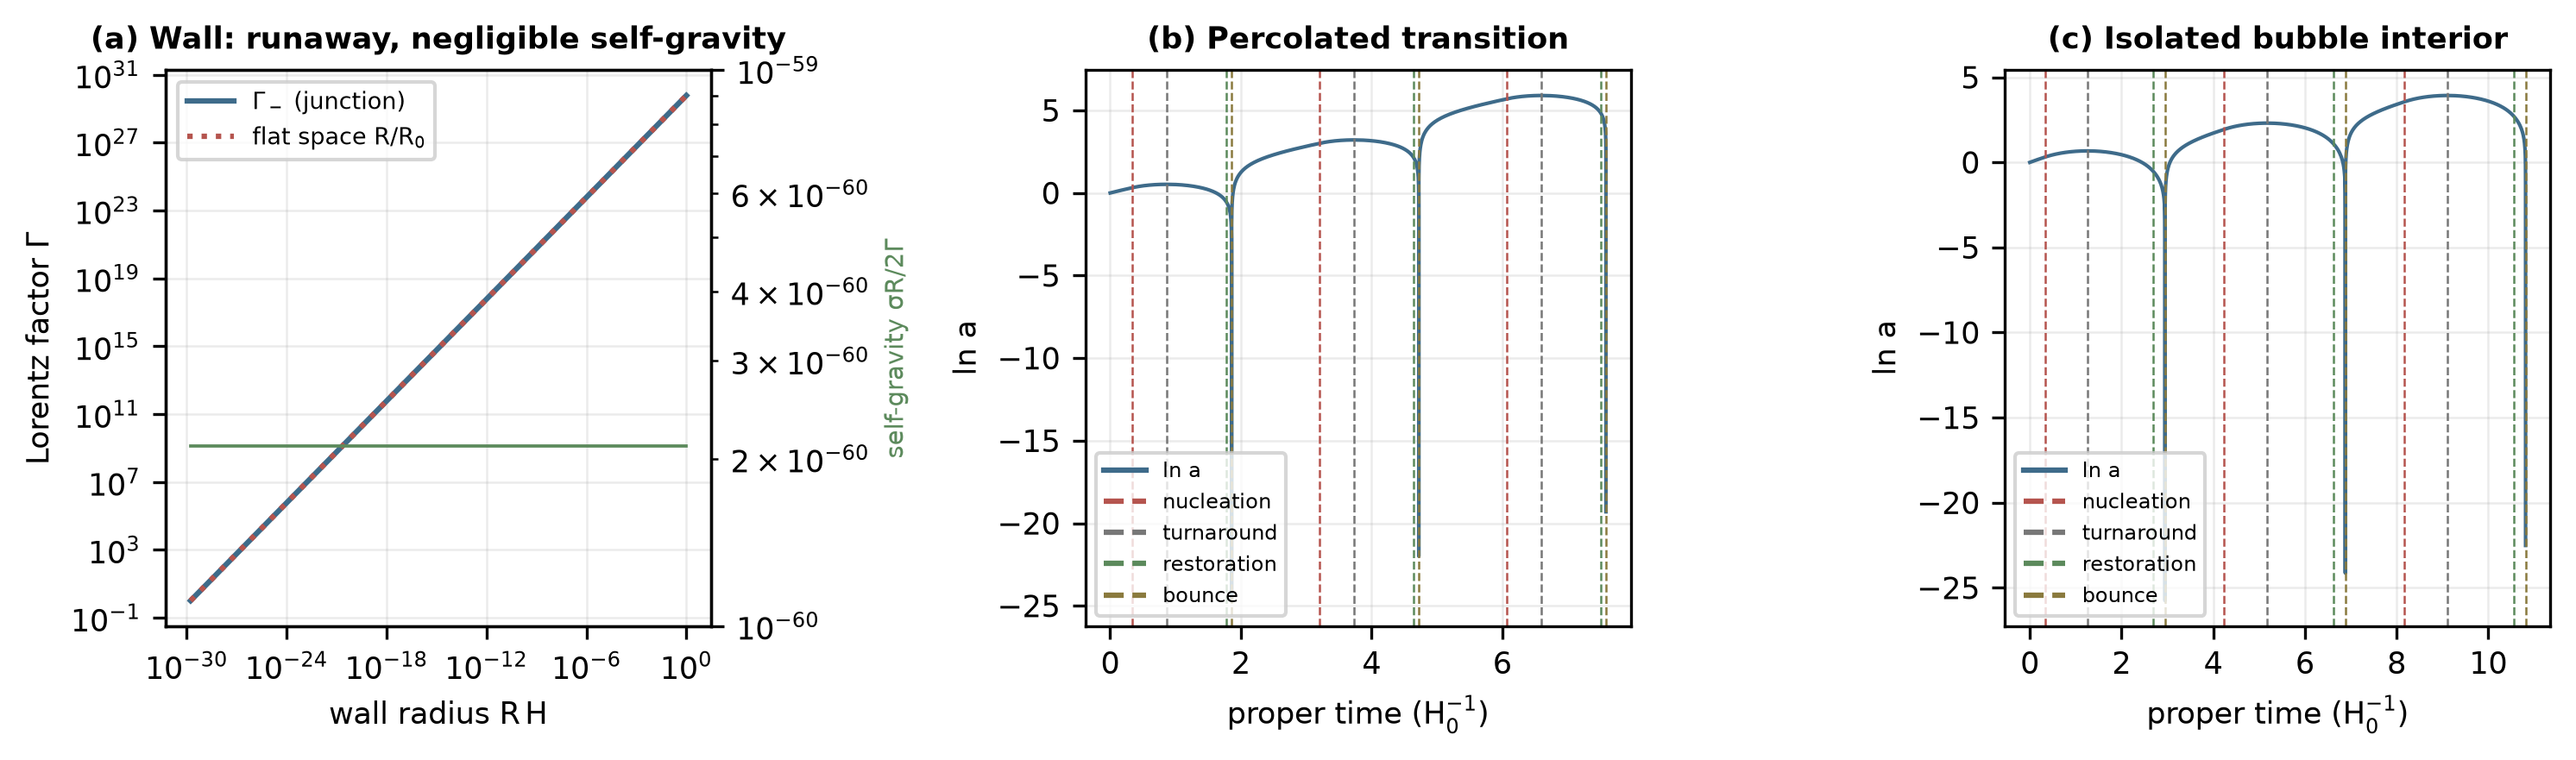
\includegraphics[width=1.00\textwidth]{../figures/fig5_daughter_evolution.png}\caption{(a) Lorentz factor of the wall from the Israel junction against the flat-space runaway, and its self-gravity (right axis). (b) Scale factor of a transitioned region continued formally through an effective bounce (the conditional continuation of Section 7.3, not supported by the dark matter of Section 3). (c) The same equations for the open region enclosed by an isolated Hubble-scale bubble, which becomes trapped before its restoration (Section 7.2).}\end{figure}
\section{Energy accounting and the fate of the transitioned region}
\subsection{The region enclosed by the wall}
A wall says nothing by itself about the cosmology inside it; the interior has to be solved. It is evolved as a Friedmann region with radiation, baryons, dark matter of field-dependent mass $A(x)$ and the scalar in one of its minima: the scalar mass, of order meV, exceeds $H$ by thirty orders of magnitude, so the field follows its minimum adiabatically, and the stress-energy is $\rho=\rho_r+\rho_b+\rho_*+U$, $\rho+P=\frac43\rho_r+\rho_b+\rho_*A(x)$, with $U(x,\theta)$ the vacuum energy including the coupling energy $\rho_*(A-1)$. The junction fixes the initial data: the fluid inside keeps the Hubble rate of the parent at nucleation while its density drops by $\Delta V_{\rm eff}$, so an isolated Hubble-scale bubble encloses an open region with $K/a^2=\Delta V_{\rm eff}/3$, and a completed transition leaves a flat region whose wall energy is released at the collisions. Events (nucleation, turnaround, restoration) are found as roots in $\ln a$ with $H$ from the constraint, so the constraint holds exactly between events; an independent integration as an initial-value problem reproduces the turnaround and the restoration to $2\times10^{-11}$ in time with a constraint residual of $2\times10^{-12}$.

In the environmental picture of Section 4.4 the transitioned volume is a network of voids and, later, sheets and filaments, which together fill most of space, while the haloes keep the held vacuum. Its volume-averaged vacuum energy is negative once it fills most of space, and a region in which the transition is complete holds the negative true vacuum, turns around at 1.23 times the scale factor at nucleation and contracts. When the dark-matter density in the contraction reaches $\theta_{\rm high}$ the true minimum disappears and the field returns to the matter-held minimum, releasing $0.75\,V_f$; the matter term restores the held vacuum, a direct consequence of the density dependence. This restoration needs dissipation: undamped, the oscillation about the held minimum is an adiabatic invariant that returns to the same amplitude when the density falls back through $\theta_{\rm high}$. The inhomogeneous evolution of a universe with islands of the held vacuum is not computed here; the volume-averaged statement is that it recollapses. With the dark-matter energy of a sudden crossing (Section 5; region\_sensitivity.py) the turnaround moves from 1.229 to 1.236 times the nucleation scale factor and the restoration happens earlier in the contraction; part of that energy is kinetic and redshifts away, so the two values bracket the evolution.

\subsection{Isolated Hubble-scale bubbles develop trapped surfaces}
A bubble that remains isolated on the Hubble scale, which happens when the transition does not complete, encloses an open region that also turns around (at 1.43 times the nucleation scale factor), but its continuation is not part of the parent universe. Following the wall as a null ray in the open interior and comparing the Misner--Sharp mass inside it with that of the exterior false-vacuum universe at the same areal radius, the interior becomes a trapped region ($\rho_{\rm in}R^2/3>1$) at $t=2.48/H_0$ and denser than the exterior at $t=2.56/H_0$, both before its restoration ($2.70$) and before any bounce ($2.95$) (Fig. 8b). Within the thin-wall junction model the interior then contains a trapped surface, an apparent horizon, and the junction requires $\Gamma_+$ to change sign, as for the false-vacuum bubbles of [17, 18, 19]. Whether a global event horizon forms, and hence a black hole, depends on the subsequent evolution, which is not computed. The trapping time does not depend on the exterior cosmology (it is unchanged for $\Omega_\Lambda\pm0.02$ and with the coupling energy of the held vacuum in the exterior) and moves to 2.32 when the dark matter receives the sudden-crossing energy, still before the restoration (2.57) and the bounce (2.85) of that run (region\_sensitivity.py). Void-sized regions, much smaller than the Hubble radius, are not trapped in this way: their trapping parameter is smaller by $(R_{\rm void}H)^2\sim10^{-4}$, and they follow the averaged evolution.

\begin{figure}[htbp]\centering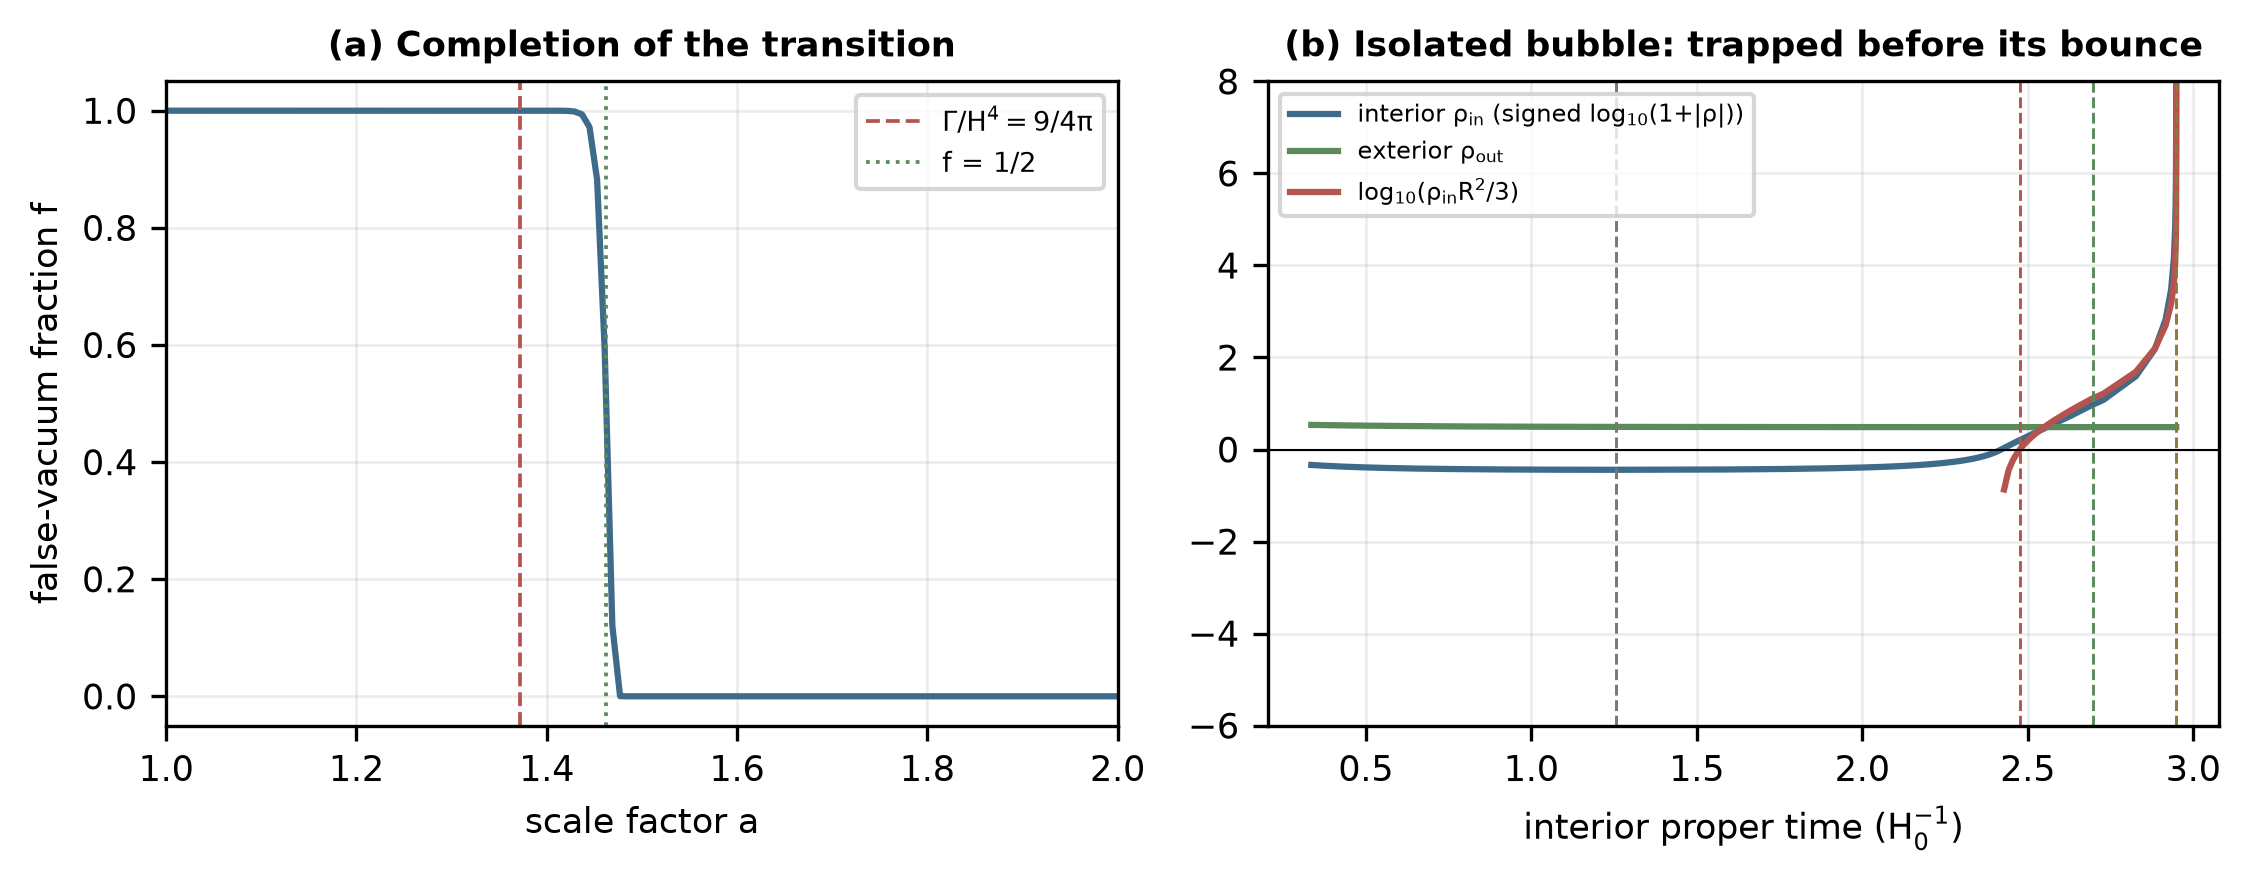
\includegraphics[width=1.00\textwidth]{../figures/fig6_handoff.png}\caption{(a) Fraction of space in the false vacuum along the dilution history of a connected region, with the completion criterion $\Gamma/H^4=9/4\pi$. (b) Isolated Hubble-scale bubble: density inside the wall and in the exterior, and the trapping parameter $\rho_{\rm in}R^2/3$, with the turnaround, restoration and bounce of the interior.}\end{figure}
\subsection{Energy and entropy closure, and why a continuation is not supported}
Every species crosses the wall, so the comoving entropy of the region is inherited, and it is raised when the wall energy is thermalized at the collisions (by a factor of approximately 3098) and when the vacuum is restored (bubble\_entropy.py); it never decreases. The interior bookkeeping $dE_{\rm in}=F_E\,dV+W_{\rm wall}$, with the swept-in content $F_E=\rho_+$ and the work $W_{\rm wall}=-\Delta V_{\rm eff}dV$ handed to the wall, closes to round-off. The decay removes the cosmological horizon of the false vacuum, whose entropy ($3.3\times10^{122}$) exceeds that of the radiation in a Hubble volume ($5.4\times10^{88}$); this is the usual situation for decays out of de Sitter space, accounted for by the action itself.

The collision products are not computed; their equation of state is bracketed: if they behave as radiation the region evolves exactly as with thermalized wall energy, and if they are massive scalar quanta ($w=0$) the turnaround moves from 1.22 to 1.29 times the nucleation scale factor. Whether the recollapsing region could be continued through a nonsingular bounce into a new cycle is a separate question. With an effective loop-quantum-cosmology bounce [32, 33] the equations do repeat, self-similarly with growth $\ln G=2.683$ per cycle ($1.622$ for $w=0$ products), but only if the bounce returns the dark matter to the state that holds the vacuum in the next cycle. For a thermal relic a hot bounce does that through freeze-out; for the wave dark matter that Section 3 requires it does not, because a meV-scale boson thermalized at a hot bounce is a hot relic, not a cold coherent condensate. The dark matter that allows the trigger is therefore not the dark matter that would allow a cyclic continuation, and the latter is not supported in this branch.

\section{Parameter-space analysis and numerical controls}
Controls separate the contribution of each ingredient (bubble\_to\_cycle.py, granularity.py; Table 4). Without the coupling (D) there is no density dependence, and a single transition that has neither already happened in our past light cone nor fails to complete requires $B_0$ in a window of width 3 around 288. With the coupling but a granular source, particle dark matter or wave dark matter lighter than the field, the rate is the zero-density rate, and the vacuum decays in the past. With the computed transmission (C) the region is identical to that with every species transmitted (B) to $2\times10^{-88}$: the selectivity of the wall changes nothing, and a hypothetical wall that keeps all dark matter out (C*) differs only in the conditional continuation.

\begin{table}[htbp]\centering\small
\caption{Controls ($\eta=0.30$, $q=1$, $B_0=200$; voids at 10\% of the mean density).}
\begin{tabular}{>{\raggedright\arraybackslash}p{0.131\dimexpr\textwidth-10\tabcolsep\relax}>{\raggedright\arraybackslash}p{0.297\dimexpr\textwidth-10\tabcolsep\relax}>{\raggedright\arraybackslash}p{0.173\dimexpr\textwidth-10\tabcolsep\relax}>{\raggedright\arraybackslash}p{0.268\dimexpr\textwidth-10\tabcolsep\relax}>{\raggedright\arraybackslash}p{0.131\dimexpr\textwidth-10\tabcolsep\relax}}
\toprule
Model & Description & Release & Past light cone & Outcome \\ \midrule
D & no matter coupling & constant rate & window $286\le B_0\le289$ & fine tuning \\
G1 & coupling, particle dark matter & zero-density rate between particles & $e^{86}$ bubbles in the past & excluded \\
G2 & coupling, wave dark matter $m_{\rm dm}\ll m_\varphi$ & zero-density rate at the nodes & as G1 & excluded \\
B & coupling, wave dark matter in the window, all species transmitted & local mean field & past clear in voids for $\bar\theta_0\gtrsim1.0\,\theta_{\rm deg}$ & viable \\
C & as B with the computed transmission & local mean field & identical to B & viable \\
C* & fully selective wall (hypothetical) & local mean field & differs only in a continuation & -- \\
\bottomrule
\end{tabular}
\end{table}
In the plane of $B_0$ and the local coupling today in the emptiest regions, the region in which the past light cone is clear and the transition completes extends from $B_0=100$ to $280$ for suitable couplings and covers 32\% of the plane scanned (Fig. 9); above the upper end the vacuum rate itself is too small for completion. A survey over stated ranges (viability\_mc.py; 3000 draws, log-uniform $B_0\in[50,1000]$, local $\theta_0/\theta_{\rm deg}\in[10^{-3},10]$, uniform $q\in[-1,3]$, $\eta\in\{0.20,0.30,0.36\}$) finds a clear past light cone in 68\% of draws, completion in 57\% and a negative true vacuum, needed for recollapse, in 75\%; the three hold together in 19\%. These fractions describe the sample space of the model, not a probability for our universe, and they presuppose the wave dark matter of Section 3; for particle dark matter the fraction is zero.

These fractions depend on the sampling distributions and do not yet include the conditions of Sections 3 and 5. An extended survey (viability\_extended.py; two sets of 3000 draws) adds the dark-matter mass, the depth of the emptiest regions and the runaway of the wall with the sudden-crossing energy, and evaluates every condition in the emptiest regions. With broad distributions (log-uniform $B_0\in[50,1000]$, local $\theta_0/\theta_{\rm deg}\in[10^{-3},10]$, $q\in[-1,3]$, $1+\delta_v\in[0.05,0.5]$, $m_{\rm dm}$ from 1 $\mu$eV to 1 GeV) the background conditions hold in 20\% of draws, adding the mean-field condition ($5m_\varphi\le m_{\rm dm}\le m_{\rm cl}$) leaves 1.3\%, and adding the runaway leaves 0.53\%; with distributions concentrated on the region of interest ($B_0\in[150,400]$, $q\in[0.1,3]$, $m_{\rm dm}$ from 1 meV to 1 eV) the fractions are 41\%, 14\% and 12\%. The joint fraction varies little with the depth of the emptiest regions (0.3--0.7\% across the terciles of the broad set). The mean-field condition is the binding one; the aim is not a large fraction but a region that survives every condition, and it does (Table S9).

All 40 checks of interface\_validation.py pass (Table S1): the analytic degeneracy and window edges, the kink tension and thickness, the bounce actions against an independent table, the thin-wall limit, shooting against collocation, the transmission against Poeschl--Teller and the sharp step, unitarity and tolerance convergence, the flat-space limit of the junction and the energy carried by the wall, the constraint and continuity of the region evolution, entropy monotonicity, the controls, the completion time and the independent integration. The granularity estimates (granularity.py) and the resolved tests (granular\_field.py, wave\_wall\_1d.py) are tabulated with their convergence checks in Tables S4--S8.

\begin{figure}[htbp]\centering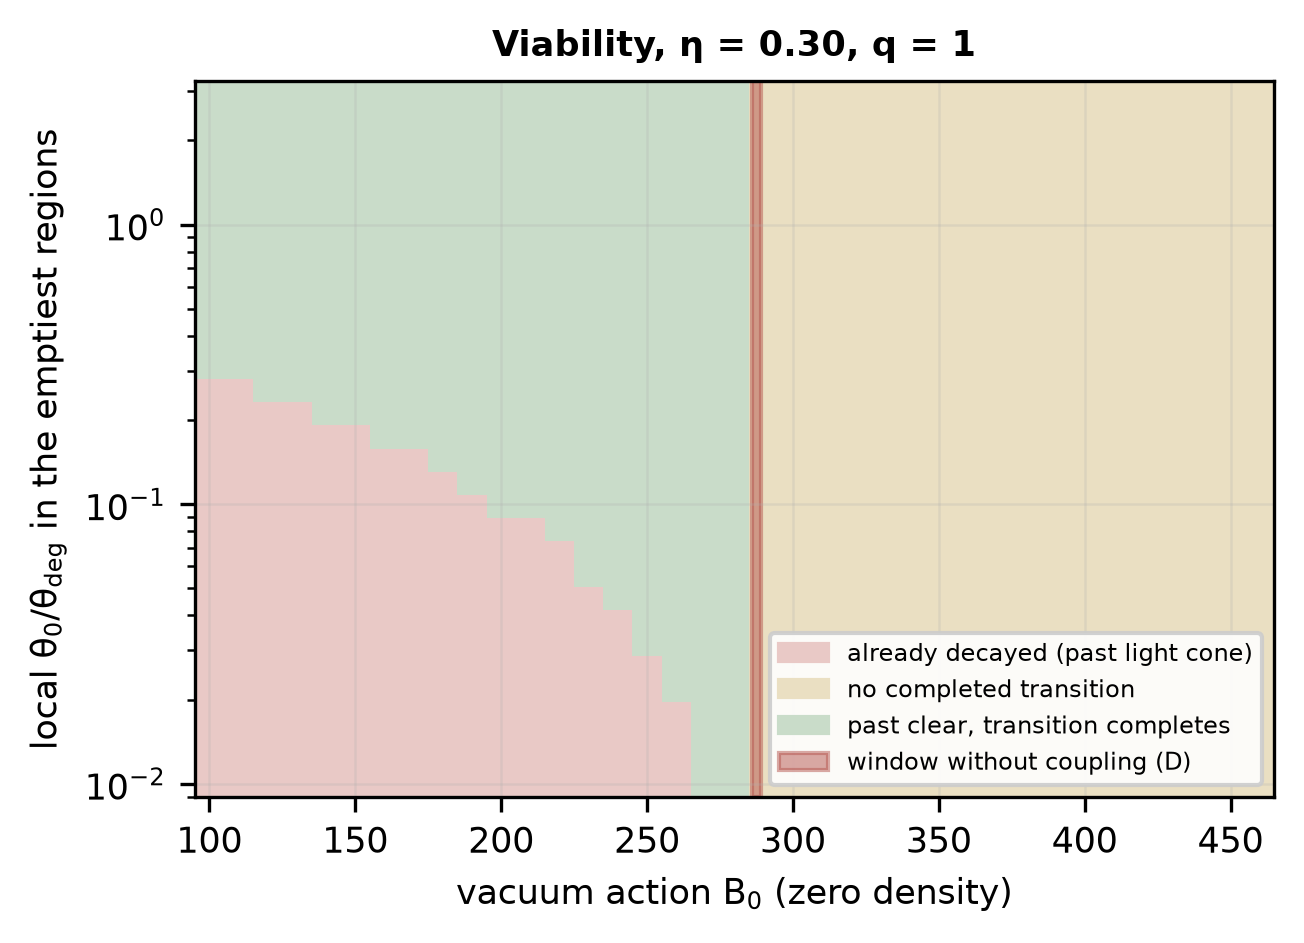
\includegraphics[width=0.73\textwidth]{../figures/fig7_viability_map.png}\caption{Outcome over the vacuum action $B_0$ and the local coupling today in the emptiest regions ($\eta=0.30$, $q=1$): already decayed in the past light cone, no completed transition, or a completed transition; the red band is the window without coupling (D).}\end{figure}
\section{An optional neutrino--scalar coupling}
The dark-matter-only model makes no prediction for neutrinos. If the scalar also coupled to neutrinos, a new hypothesis, the neutrino masses would track the local field. As an illustrative benchmark consider a flavour-universal Dirac coupling $\mathcal L=-y\varphi\bar\nu\nu$, which requires an electroweak completion (for instance a higher-dimensional operator with the Higgs field and right-handed neutrinos) that is not specified here; the masses shift by $\delta m_\nu=yfx_{\rm loc}$, with $x_{\rm loc}$ the held minimum at the local dark-matter coupling (neutrino\_coupling.py).

Terrestrial oscillation experiments would see none of it. The scalar couples to dark matter only, and at the dark-matter density of the solar neighbourhood, approximately $2.4\times10^{5}$ times the cosmic mean, the field sits at $1-x=1.4\times10^{-6}$. Along a 1300 km baseline such as that of DUNE [34], and along the baselines of Hyper-Kamiokande [35], the halo density changes by a relative $1\times10^{-14}$ and the field by less than $10^{-15}$. The shift is then a constant addition to the mass matrix, absorbed into the measured masses and mixing, so that $\Delta P_{\alpha\beta}(E)=0$ identically; an interface, across which a neutrino would accumulate a different oscillation phase, does not exist inside a protected past light cone. This null result is itself a constraint: a terrestrial signal of a scalar-dependent neutrino mass would not come from this model.

The coupling would instead make the neutrino masses depend on environment and on time, as in mass-varying-neutrino models [36]. Relative to the solar neighbourhood the masses would be smaller by $0.35y$ meV at the mean density and $0.58y$ meV in the deepest voids today, and the mean-density value would be larger by $0.35y$ meV at recombination than today (Table 5). For a perturbative coupling these shifts are below a meV, beneath the sensitivity of present cosmological and laboratory mass measurements; a larger coupling would need a separate assessment of neutrino self-interaction and free-streaming constraints, which is not attempted. Relic neutrinos also act back on the trigger, adding $n_\nu m_\nu(\varphi)$ to the effective potential, a tilt $\delta\eta=8.9\times10^{-5}\,y$, so the trigger is unaffected for $y\lesssim34$ (a shift of 1\% of $\eta$). Inside a transitioned region the masses would shift by $-5.6y$ meV. Neutrino production in wall collisions and a neutrino-driven trigger are separate questions and are not addressed.

\begin{table}[htbp]\centering\small
\caption{Optional neutrino coupling: the held minimum and the neutrino-mass shift per unit coupling relative to the solar neighbourhood ($\bar\theta_0=3\,\theta_{\rm deg}$).}
\begin{tabular}{llll}
\toprule
Environment & $1+\delta$ & $x_{\rm loc}$ & $\delta m_\nu/y$ (meV) \\ \midrule
deepest voids (10\% of mean) & 0.1 & 0.8059 & -0.577 \\
mean density & 1 & 0.8829 & -0.348 \\
galactic halo (200x mean) & 200 & 0.9984 & -0.005 \\
solar neighbourhood & $2.4\times10^{5}$ & 1.0000 & 0.000 \\
mean density at $z=1$ & -- & 0.9670 & -0.098 \\
mean density at $z=3$ & -- & 0.9950 & -0.015 \\
mean density at $z=1100$ & -- & 1.0000 & +0.000 \\
\bottomrule
\end{tabular}
\end{table}
\section{Implications, limitations and conclusions}
A coupling of a scalar to dark matter centered on a false vacuum makes the stability of that vacuum a function of the dark-matter density, and dilution turns the held vacuum from the true into a metastable one at $\theta_{\rm deg}=\eta/2$. For a vacuum at the dark-energy scale this mean-field statement holds only if the dark matter looks smooth to the field on a scale below a tenth of a millimeter and a time below a picosecond. In a spatially resolved treatment particle dark matter does not, and with it the vacuum decays at its zero-density rate; the coincidence of the dark-matter and dark-energy densities, which motivates a dilution trigger, is what makes it fail. Wave dark matter heavier than the field and still classical, roughly 3 meV to 0.25 eV, does, and then the decay is environmental. It begins in the emptiest voids, the past is protected only if the mean coupling today is close to the degeneracy density, the transition advances from voids into sheets and filaments as the universe expands, and galactic haloes keep the held vacuum. Within the voids the wall is a fraction of a millimeter thick, runs away, becomes transparent to the dark matter and carries the released energy, while the dark matter it crosses is kicked forward and trails it; transitioned regions recollapse in their negative vacuum, and isolated Hubble-scale bubbles develop trapped surfaces.

The observational implications follow from the environment. The dark energy measured inside haloes is unchanged until the global recollapse, so local tests see none of the transition, while the volume-averaged expansion responds to the voids. The dark matter must be a nonthermal boson in the meV to sub-eV range with a coupling to the scalar of strength $M\approx f$, which changes its mass by a factor 2.7 between the vacua; such a coupling acts only over the Compton length of the scalar and is invisible to astrophysical fifth-force tests. The dark energy is exactly $w=-1$ until the trigger, and the order of the future transition follows the density of the cosmic web, $a_{\rm tr}\propto(1+\delta)^{1/3}$. Within the resolved treatment of Section 3.5, a detection of thermal-relic dark matter, or of dark matter heavier than about an eV, would exclude the density-triggered decay of a dark-energy-scale vacuum in this class of models.

The limitations are specific. The granular decay rate is computed at first order in each source's coupling with static sources and an undeformed bounce, which overstates the suppression and so does not weaken the conclusion for particle dark matter, but it is not a fully four-dimensional inhomogeneous bounce. The wave-dark-matter crossing is simulated in 1+1 dimensions for a planar wall, not for an expanding bubble. The local density is treated as constant along the past light cone of a region, which is conservative for voids; the void statistics enter only through the depth of the emptiest regions; the advance of the walls into denser regions and the islands of held vacuum are described through the degeneracy contour, not simulated; and the trapped surfaces of isolated bubbles are found within the thin-wall junction model, without establishing a global event horizon. The one-loop prefactor is estimated, not computed, and enters the completion time only logarithmically; the collision products are bracketed by their equation of state; and the next-to-leading friction is estimated for a hypothetical dark gauge boson only.

The results do not require a cosmological bounce, and they do not support one in this branch. They establish when a density-dependent vacuum can decay at all, where it decays first, what its walls transmit and how they move, and what the regions they enclose become. The homogeneous, classical version of the trigger, which does not face the granularity bound because its field has a cosmological Compton length, is examined in the companion paper [20].

\section*{Declarations}
\noindent\textbf{Funding.} This research received no specific grant from funding agencies in the public, commercial, or not-for-profit sectors.

\noindent\textbf{Declaration of competing interest.} The author declares no known competing financial interests or personal relationships that could have influenced the work reported in this paper.

\noindent\textbf{CRediT authorship contribution statement.} Leon Sandler: Conceptualization, Methodology, Software, Formal analysis, Investigation, Writing -- original draft, Writing -- review and editing.

\noindent\textbf{Data and code availability.} All code (Python, NumPy, SciPy, Matplotlib [37, 38]) and the data behind every figure and table are at \url{https://github.com/sandlerleon/matter-coupled-vacuum-bubbles} (MIT license) and archived at \url{https://doi.org/10.5281/zenodo.23841878}; this manuscript is archived at \url{https://doi.org/10.5281/zenodo.23841874}. Input tables shared with the companion paper are documented as such in the README.

\noindent\textbf{Related manuscript.} A companion manuscript on the homogeneous version of the trigger and its continuation into cycles has been prepared for The European Physical Journal C, archived at \url{https://doi.org/10.5281/zenodo.23841870}; it shares the class of models but none of the results reported here.

\noindent\textbf{Declaration of generative AI and AI-assisted technologies in the writing process.} During the preparation of this work the author used Claude (Anthropic) to assist with the numerical analysis, code, literature checking and drafting. After using this tool, the author reviewed and edited the content as needed and takes full responsibility for the content of the publication.

\section*{References}
\noindent\hangindent=1.5em [1] S. Coleman, Fate of the false vacuum: Semiclassical theory. Phys. Rev. D 15, 2929--2936 (1977). \url{https://doi.org/10.1103/PhysRevD.15.2929}\par
\noindent\hangindent=1.5em [2] C.G. Callan, S. Coleman, Fate of the false vacuum. II. First quantum corrections. Phys. Rev. D 16, 1762--1768 (1977). \url{https://doi.org/10.1103/PhysRevD.16.1762}\par
\noindent\hangindent=1.5em [3] S. Coleman, F. De Luccia, Gravitational effects on and of vacuum decay. Phys. Rev. D 21, 3305--3315 (1980). \url{https://doi.org/10.1103/PhysRevD.21.3305}\par
\noindent\hangindent=1.5em [4] J. Khoury, A. Weltman, Chameleon fields: awaiting surprises for tests of gravity in space. Phys. Rev. Lett. 93, 171104 (2004). \url{https://doi.org/10.1103/PhysRevLett.93.171104}\par
\noindent\hangindent=1.5em [5] K. Hinterbichler, J. Khoury, Screening long-range forces through local symmetry restoration. Phys. Rev. Lett. 104, 231301 (2010). \url{https://doi.org/10.1103/PhysRevLett.104.231301}\par
\noindent\hangindent=1.5em [6] K. Hinterbichler, J. Khoury, A. Levy, A. Matas, Symmetron cosmology. Phys. Rev. D 84, 103521 (2011). \url{https://doi.org/10.1103/PhysRevD.84.103521}\par
\noindent\hangindent=1.5em [7] L. Amendola, Coupled quintessence. Phys. Rev. D 62, 043511 (2000). \url{https://doi.org/10.1103/PhysRevD.62.043511}\par
\noindent\hangindent=1.5em [8] G. Isidori, G. Ridolfi, A. Strumia, On the metastability of the Standard Model vacuum. Nucl. Phys. B 609, 387--409 (2001). \url{https://doi.org/10.1016/S0550-3213(01)00302-9}\par
\noindent\hangindent=1.5em [9] J.R. Espinosa, G.F. Giudice, A. Riotto, Cosmological implications of the Higgs mass measurement. J. Cosmol. Astropart. Phys. 2008(05), 002 (2008). \url{https://doi.org/10.1088/1475-7516/2008/05/002}\par
\noindent\hangindent=1.5em [10] R. Bousso, J. Polchinski, Quantization of four-form fluxes and dynamical neutralization of the cosmological constant. J. High Energy Phys. 2000(06), 006 (2000). \url{https://doi.org/10.1088/1126-6708/2000/06/006}\par
\noindent\hangindent=1.5em [11] B. Freivogel, M. Kleban, M. Rodriguez Martinez, L. Susskind, Observational consequences of a landscape. J. High Energy Phys. 2006(03), 039 (2006). \url{https://doi.org/10.1088/1126-6708/2006/03/039}\par
\noindent\hangindent=1.5em [12] M. Kleban, Cosmic bubble collisions. Class. Quantum Grav. 28, 204008 (2011). \url{https://doi.org/10.1088/0264-9381/28/20/204008}\par
\noindent\hangindent=1.5em [13] A. Aguirre, M.C. Johnson, A status report on the observability of cosmic bubble collisions. Rep. Prog. Phys. 74, 074901 (2011). \url{https://doi.org/10.1088/0034-4885/74/7/074901}\par
\noindent\hangindent=1.5em [14] M.J. Baker, J. Kopp, A.J. Long, Filtered dark matter at a first order phase transition. Phys. Rev. Lett. 125, 151102 (2020). \url{https://doi.org/10.1103/PhysRevLett.125.151102}\par
\noindent\hangindent=1.5em [15] D. Bödeker, G.D. Moore, Can electroweak bubble walls run away? J. Cosmol. Astropart. Phys. 05, 009 (2009). \url{https://doi.org/10.1088/1475-7516/2009/05/009}\par
\noindent\hangindent=1.5em [16] D. Bödeker, G.D. Moore, Electroweak bubble wall speed limit. J. Cosmol. Astropart. Phys. 05, 025 (2017). \url{https://doi.org/10.1088/1475-7516/2017/05/025}\par
\noindent\hangindent=1.5em [17] S.K. Blau, E.I. Guendelman, A.H. Guth, Dynamics of false-vacuum bubbles. Phys. Rev. D 35, 1747--1766 (1987). \url{https://doi.org/10.1103/PhysRevD.35.1747}\par
\noindent\hangindent=1.5em [18] E. Farhi, A.H. Guth, An obstacle to creating a universe in the laboratory. Phys. Lett. B 183, 149--155 (1987). \url{https://doi.org/10.1016/0370-2693(87)90429-1}\par
\noindent\hangindent=1.5em [19] E. Farhi, A.H. Guth, J. Guven, Is it possible to create a universe in the laboratory by quantum tunneling? Nucl. Phys. B 339, 417--490 (1990). \url{https://doi.org/10.1016/0550-3213(90)90357-J}\par
\noindent\hangindent=1.5em [20] L. Sandler, Matter-dilution-triggered recollapse and conditional nonsingular cycles in a metastable dark-energy model. Preprint, Zenodo (2026). \url{https://doi.org/10.5281/zenodo.23841870}\par
\noindent\hangindent=1.5em [21] S. Tremaine, J.E. Gunn, Dynamical role of light neutral leptons in cosmology. Phys. Rev. Lett. 42, 407--410 (1979). \url{https://doi.org/10.1103/PhysRevLett.42.407}\par
\noindent\hangindent=1.5em [22] L. Hui, J.P. Ostriker, S. Tremaine, E. Witten, Ultralight scalars as cosmological dark matter. Phys. Rev. D 95, 043541 (2017). \url{https://doi.org/10.1103/PhysRevD.95.043541}\par
\noindent\hangindent=1.5em [23] J. Preskill, M.B. Wise, F. Wilczek, Cosmology of the invisible axion. Phys. Lett. B 120, 127--132 (1983). \url{https://doi.org/10.1016/0370-2693(83)90637-8}\par
\noindent\hangindent=1.5em [24] S. Parke, Gravity and the decay of the false vacuum. Phys. Lett. B 121, 313--315 (1983). \url{https://doi.org/10.1016/0370-2693(83)91376-X}\par
\noindent\hangindent=1.5em [25] A.H. Guth, E.J. Weinberg, Could the universe have recovered from a slow first-order phase transition? Nucl. Phys. B 212, 321--364 (1983). \url{https://doi.org/10.1016/0550-3213(83)90307-3}\par
\noindent\hangindent=1.5em [26] M.S. Turner, E.J. Weinberg, L.M. Widrow, Bubble nucleation in first-order inflation and other cosmological phase transitions. Phys. Rev. D 46, 2384--2403 (1992). \url{https://doi.org/10.1103/PhysRevD.46.2384}\par
\noindent\hangindent=1.5em [27] G.V. Dunne, H. Min, Beyond the thin-wall approximation: Precise numerical computation of prefactors in false vacuum decay. Phys. Rev. D 72, 125004 (2005). \url{https://doi.org/10.1103/PhysRevD.72.125004}\par
\noindent\hangindent=1.5em [28] R.K. Sheth, R. van de Weygaert, A hierarchy of voids: much ado about nothing. Mon. Not. R. Astron. Soc. 350, 517--538 (2004). \url{https://doi.org/10.1111/j.1365-2966.2004.07661.x}\par
\noindent\hangindent=1.5em [29] R. Gregory, I.G. Moss, B. Withers, Black holes as bubble nucleation sites. J. High Energy Phys. 03, 081 (2014). \url{https://doi.org/10.1007/JHEP03(2014)081}\par
\noindent\hangindent=1.5em [30] P. Burda, R. Gregory, I.G. Moss, Vacuum metastability with black holes. J. High Energy Phys. 08, 114 (2015). \url{https://doi.org/10.1007/JHEP08(2015)114}\par
\noindent\hangindent=1.5em [31] W. Israel, Singular hypersurfaces and thin shells in general relativity. Nuovo Cimento B 44, 1--14 (1966). \url{https://doi.org/10.1007/BF02710419}\par
\noindent\hangindent=1.5em [32] A. Ashtekar, T. Pawlowski, P. Singh, Quantum nature of the big bang. Phys. Rev. Lett. 96, 141301 (2006). \url{https://doi.org/10.1103/PhysRevLett.96.141301}\par
\noindent\hangindent=1.5em [33] A. Ashtekar, P. Singh, Loop quantum cosmology: a status report. Class. Quantum Grav. 28, 213001 (2011). \url{https://doi.org/10.1088/0264-9381/28/21/213001}\par
\noindent\hangindent=1.5em [34] DUNE Collaboration, B. Abi et al., Deep Underground Neutrino Experiment (DUNE), Far Detector Technical Design Report, Volume II: DUNE Physics. arXiv:2002.03005 (2020).\par
\noindent\hangindent=1.5em [35] Hyper-Kamiokande Proto-Collaboration, K. Abe et al., Hyper-Kamiokande Design Report. arXiv:1805.04163 (2018).\par
\noindent\hangindent=1.5em [36] R. Fardon, A.E. Nelson, N. Weiner, Dark energy from mass varying neutrinos. J. Cosmol. Astropart. Phys. 10, 005 (2004). \url{https://doi.org/10.1088/1475-7516/2004/10/005}\par
\noindent\hangindent=1.5em [37] C.R. Harris et al., Array programming with NumPy. Nature 585, 357--362 (2020). \url{https://doi.org/10.1038/s41586-020-2649-2}\par
\noindent\hangindent=1.5em [38] P. Virtanen et al., SciPy 1.0: fundamental algorithms for scientific computing in Python. Nat. Methods 17, 261--272 (2020). \url{https://doi.org/10.1038/s41592-019-0686-2}\par

\end{document}